\documentclass[cn,pad,chinesefont=nofont,twocol,blue]{elegantbook}
\usepackage{array}
\usepackage{xpinyin}
\usepackage{latexgit}
\usepackage{hyperref}
\hypersetup{
	pdftitle={北園清箫習谱},
    pdfauthor={北园主人}
}
\setCJKmainfont{Source Han Serif} 
\setCJKsansfont{Source Han Sans} 
\setCJKmonofont{Source Han Mono}

\title{北園清箫習谱}
\author{北园主人}
\date{\zhtoday}
\cover{cover2.jpeg}
\logo{monk.png}
\extrainfo{清籁远\xpinyin*{喑}喑,秦楼夜思深。碧空人已去,沧海凤难寻。\\杳妙和云绝,依微向水沉。还将九成意,高阁伫芳音。}
\version{\gitcommithash}
\fancyfoot[C]{明月如霜,青箫独吟,小桥清溪枯柳。杯黄酒,又见纤纤酥手舞彩袖。}

\begin{document}
\maketitle
\frontmatter
\tableofcontents
\mainmatter

\chapter{箫的来历}
\paragraph*{箫,形声。字从竹从肃,肃亦声。“肃”本义为“千针万孔”,转义为“风声尖锐地漫天呼啸”。“竹”与“肃”联合起来表示“一种模拟风声漫天尖锐呼啸的竹制吹奏乐器”。本义:一种模拟风吹声的竹乐器。}
\paragraph*{箫源于远古时期的骨哨,新石器时代开始以竹制作。历史上亦称为笛,在秦汉至唐,箫是指编管的排箫。唐以后方专指竖吹之笛。“横吹笛子竖吹箫”,即笛箫之间最基本的差别。箫历史悠久,音色圆润轻柔,幽静典雅,适于独奏和重奏。} 
\paragraph*{早在《尚书·益稷》中记载有“\xpinyin*{箫韶九成,凤凰来仪}。”当因韶乐伴奏乐器以箫(当时为排箫)为主而有此称。箫在汉代时称为“\xpinyin*{篴}”、“竖篴”。西晋乐工列和、中书监荀勖所改革的笛为6 孔(前5、后1),其形制与今天的箫已非常相似了。东晋的桓伊,擅长音乐,他有一支蔡邕的柯亭笛(箫),是江南数第一的吹箫名手,地位和声望都已很高。他曾为素不相识的王徽之吹奏过三段乐曲,在历史上被传为佳话。}
\paragraph*{魏晋南北朝时,箫已用于独奏、合奏,并在伴奏相和歌的乐队中使用。清代,箫的形制完全一样。清《律吕正义后编》记载:“明时乃直曰箫,不复有竖篴。今箫长一尺八寸弱,从上口吹,有后出孔;笛横吹,无后出孔。”}
\paragraph*{当代箫有三种,分别是琴箫,洞箫和南箫。三种箫最大的区别是管径,音色稍有差异。琴箫最为细腻,南箫在稍显粗狂豪放,洞箫介于二者之间,玩转悠然。日本的尺八,是由唐尺八传到日本。后经过多年改革,并结合日本本土文化形成的日本民族乐器,音色沧桑悲凉。实际上,他们的音色差别并不大,主要是乐曲本身的特色带来的感觉。}

\paragraph*{\textbf{管径参考(mm):}\\
\begin{tabular}[t]{|c|l|l|}
  	\firsthline
           & F调           & G调 \\ \hline
    洞箫    & 外26/内18.5   & 外25/内17-18 \\
    琴箫    & 外24/内15-16  & 外23/内14-15 \\
	\lasthline 
\end{tabular}
}

\begin{center}
	\vfill
	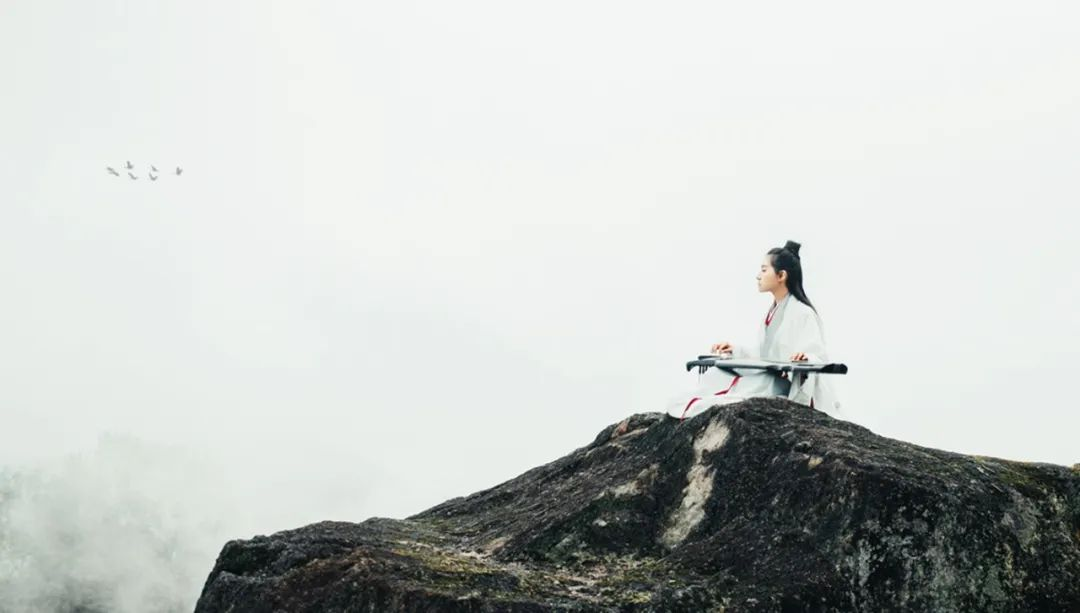
\includegraphics[width=0.5\textwidth]{cover6}
\end{center}

\chapter{指法图}
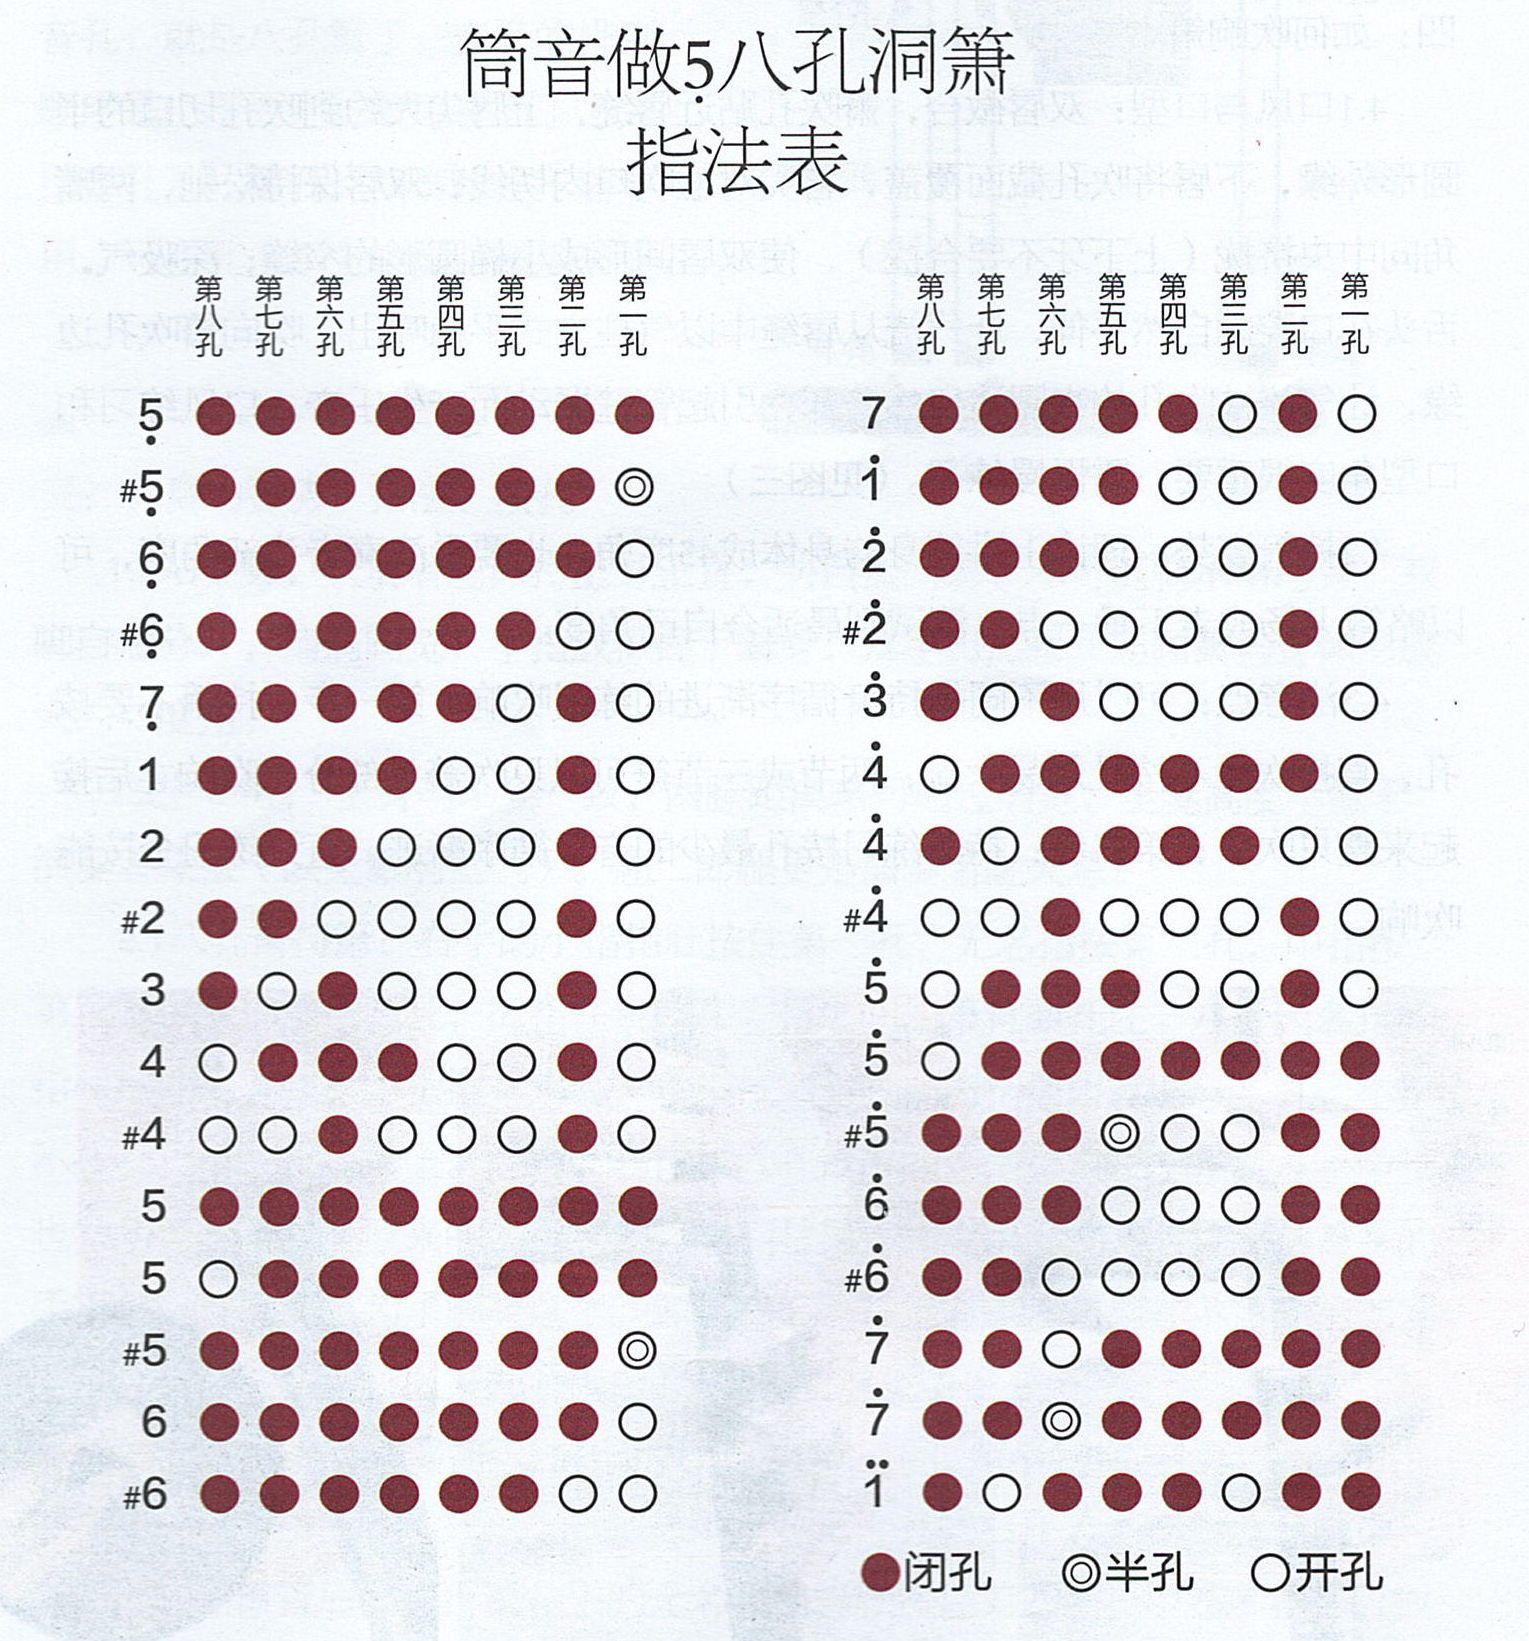
\includegraphics[width=0.93\textwidth]{dongxiao/Scan.jpeg}
\chapter{基礎谱}
\section{筒音作5}
\begin{center}
	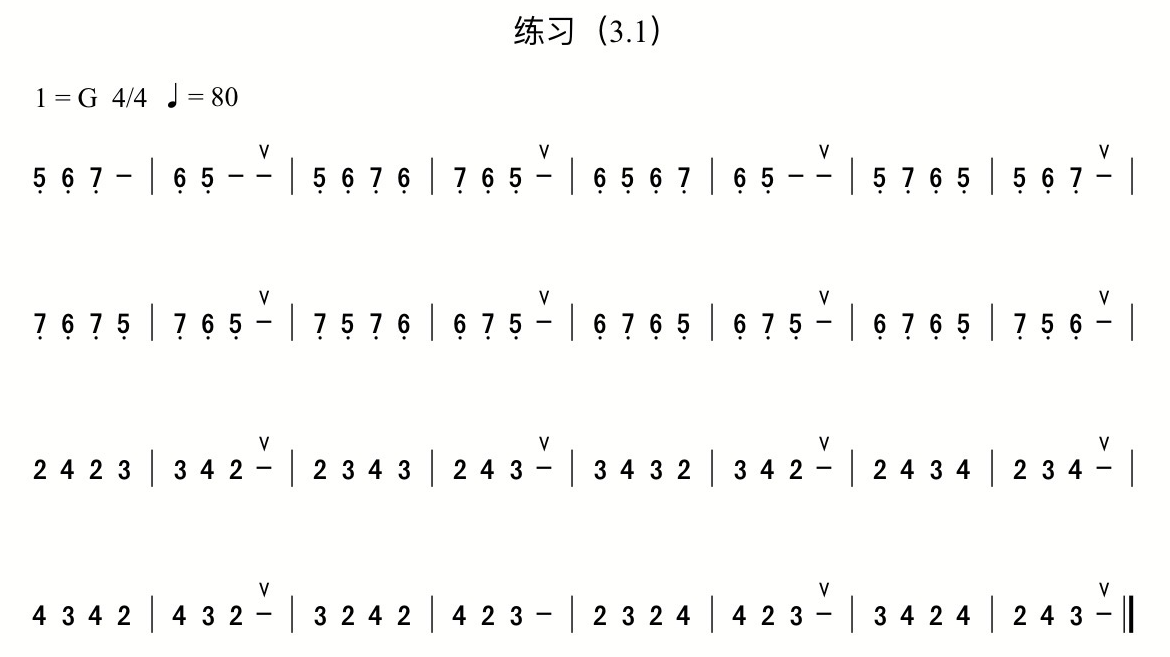
\includegraphics[width=\textwidth]{dongxiao/20200419-练习3.1.png}
\end{center}
\section{筒音作2}
	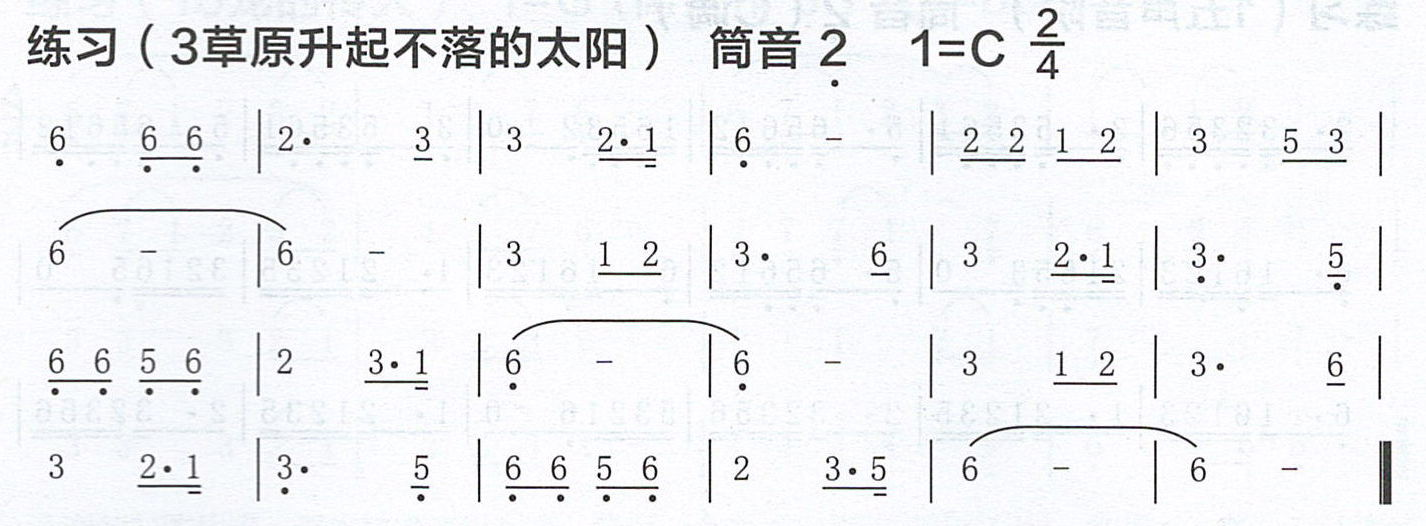
\includegraphics[width=\textwidth]{dongxiao/Scan 6.jpeg}

\chapter{首选}
\section{世上只有媽媽好}
	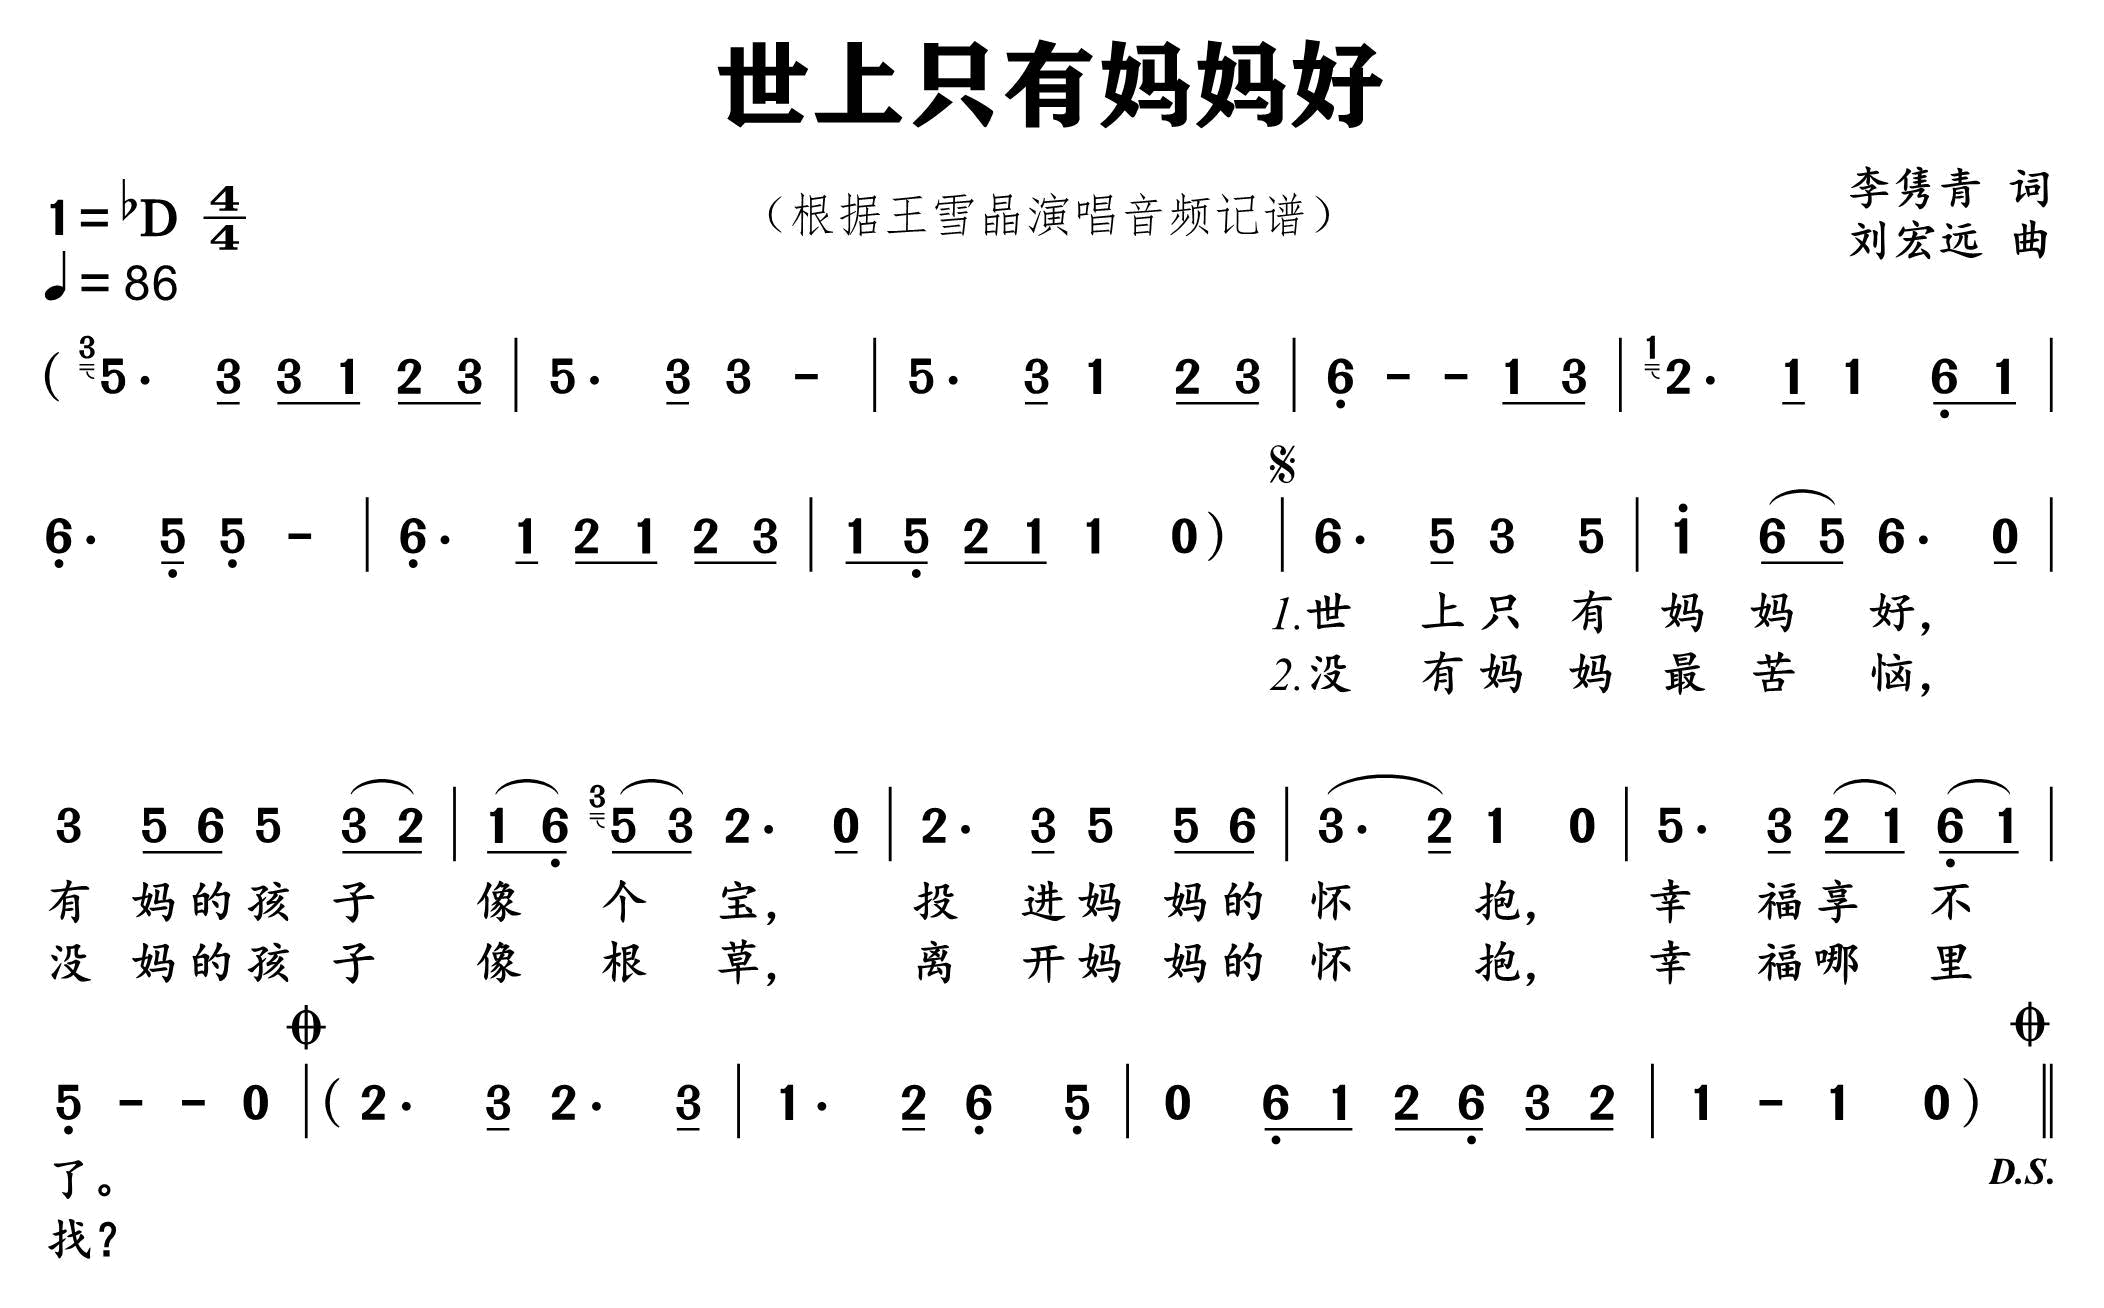
\includegraphics[width=\textwidth]{dongxiao/IMG_0854-世上只有妈妈好.png}
\section{鐘聲}
	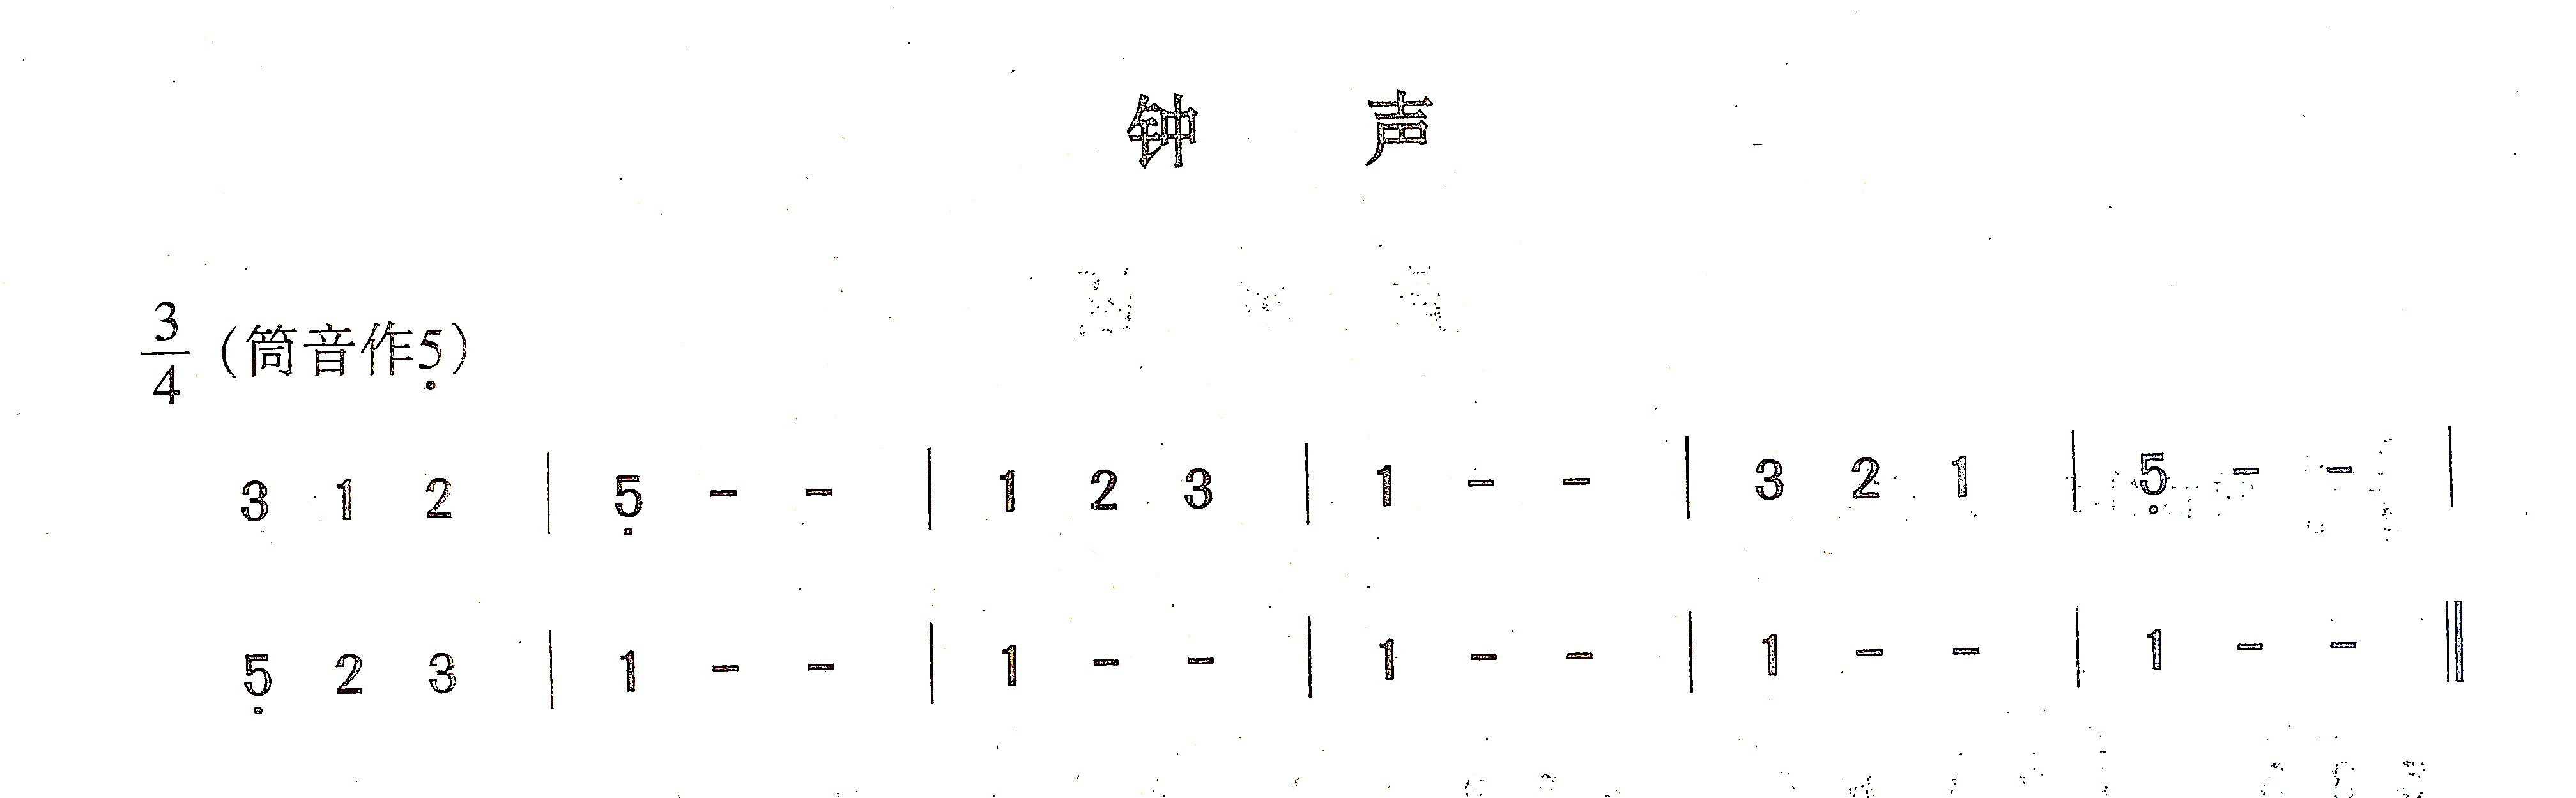
\includegraphics[width=\textwidth]{dongxiao/20200711-钟声.jpg}
\section{送別}
    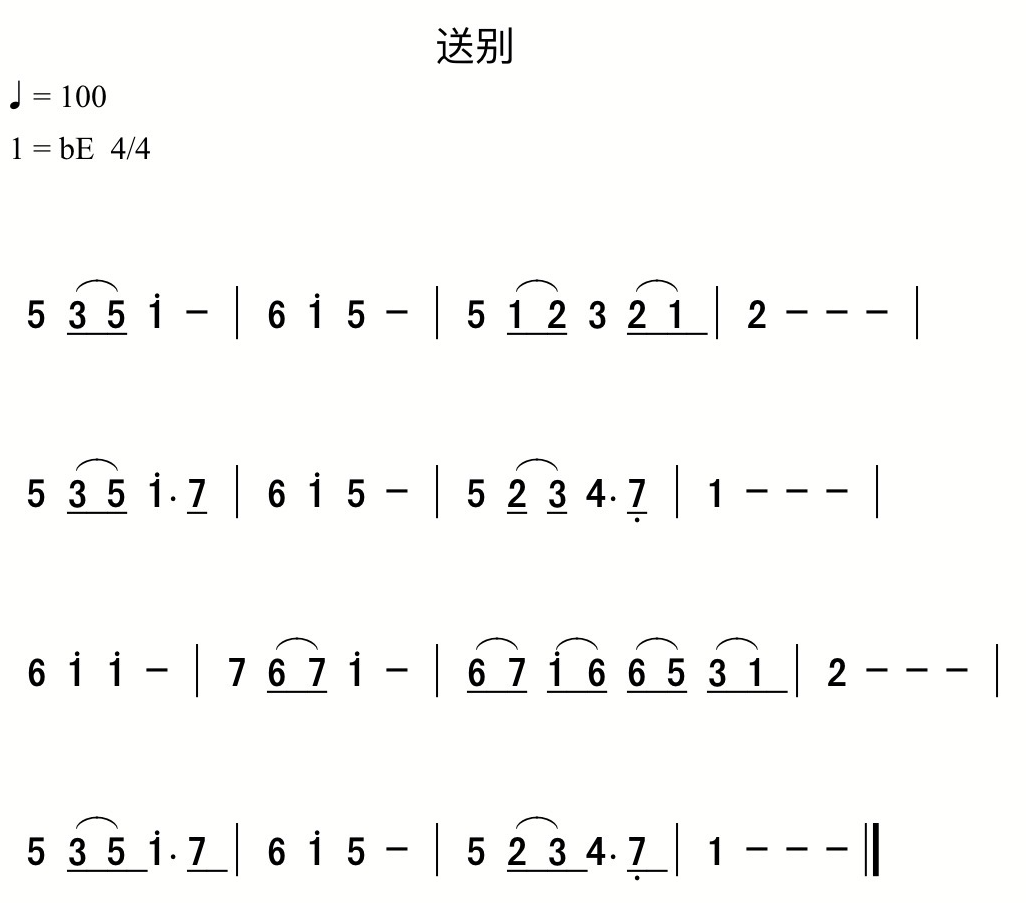
\includegraphics[width=\textwidth]{dongxiao/IMG_0855-送别.png}  
\section{兒女情}          
	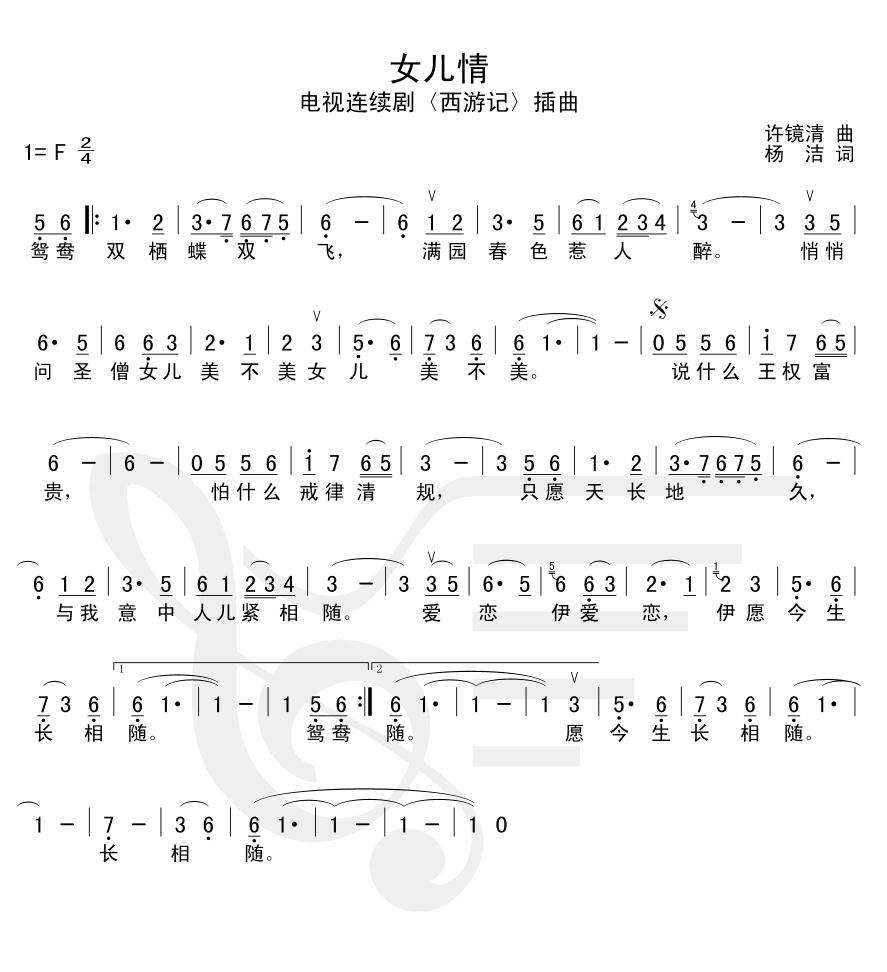
\includegraphics[width=\textwidth]{dongxiao/西游记-儿女情}  
\section{小草}
	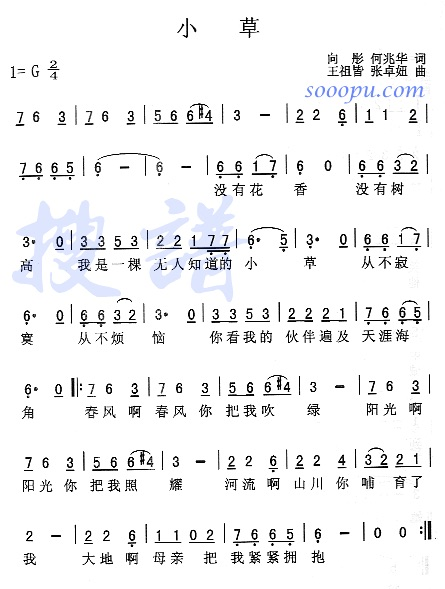
\includegraphics[width=\textwidth]{dongxiao/20200627-小草.jpg}  
\section{寒山僧蹤}
	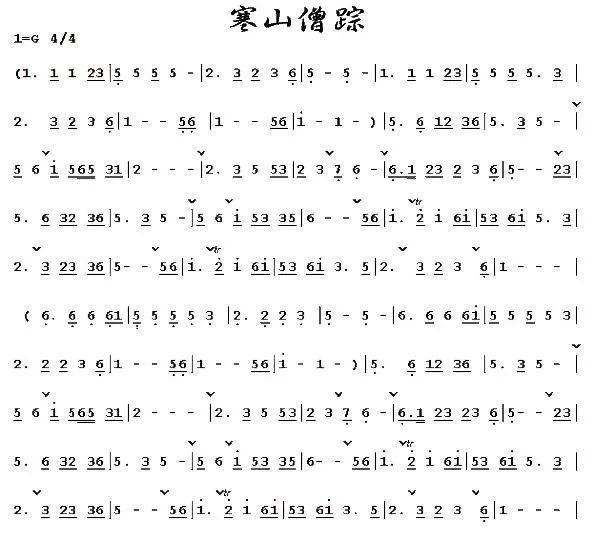
\includegraphics[width=\textwidth]{dongxiao/20200724-寒山僧踪2}  
\section{雪梅疏影}
    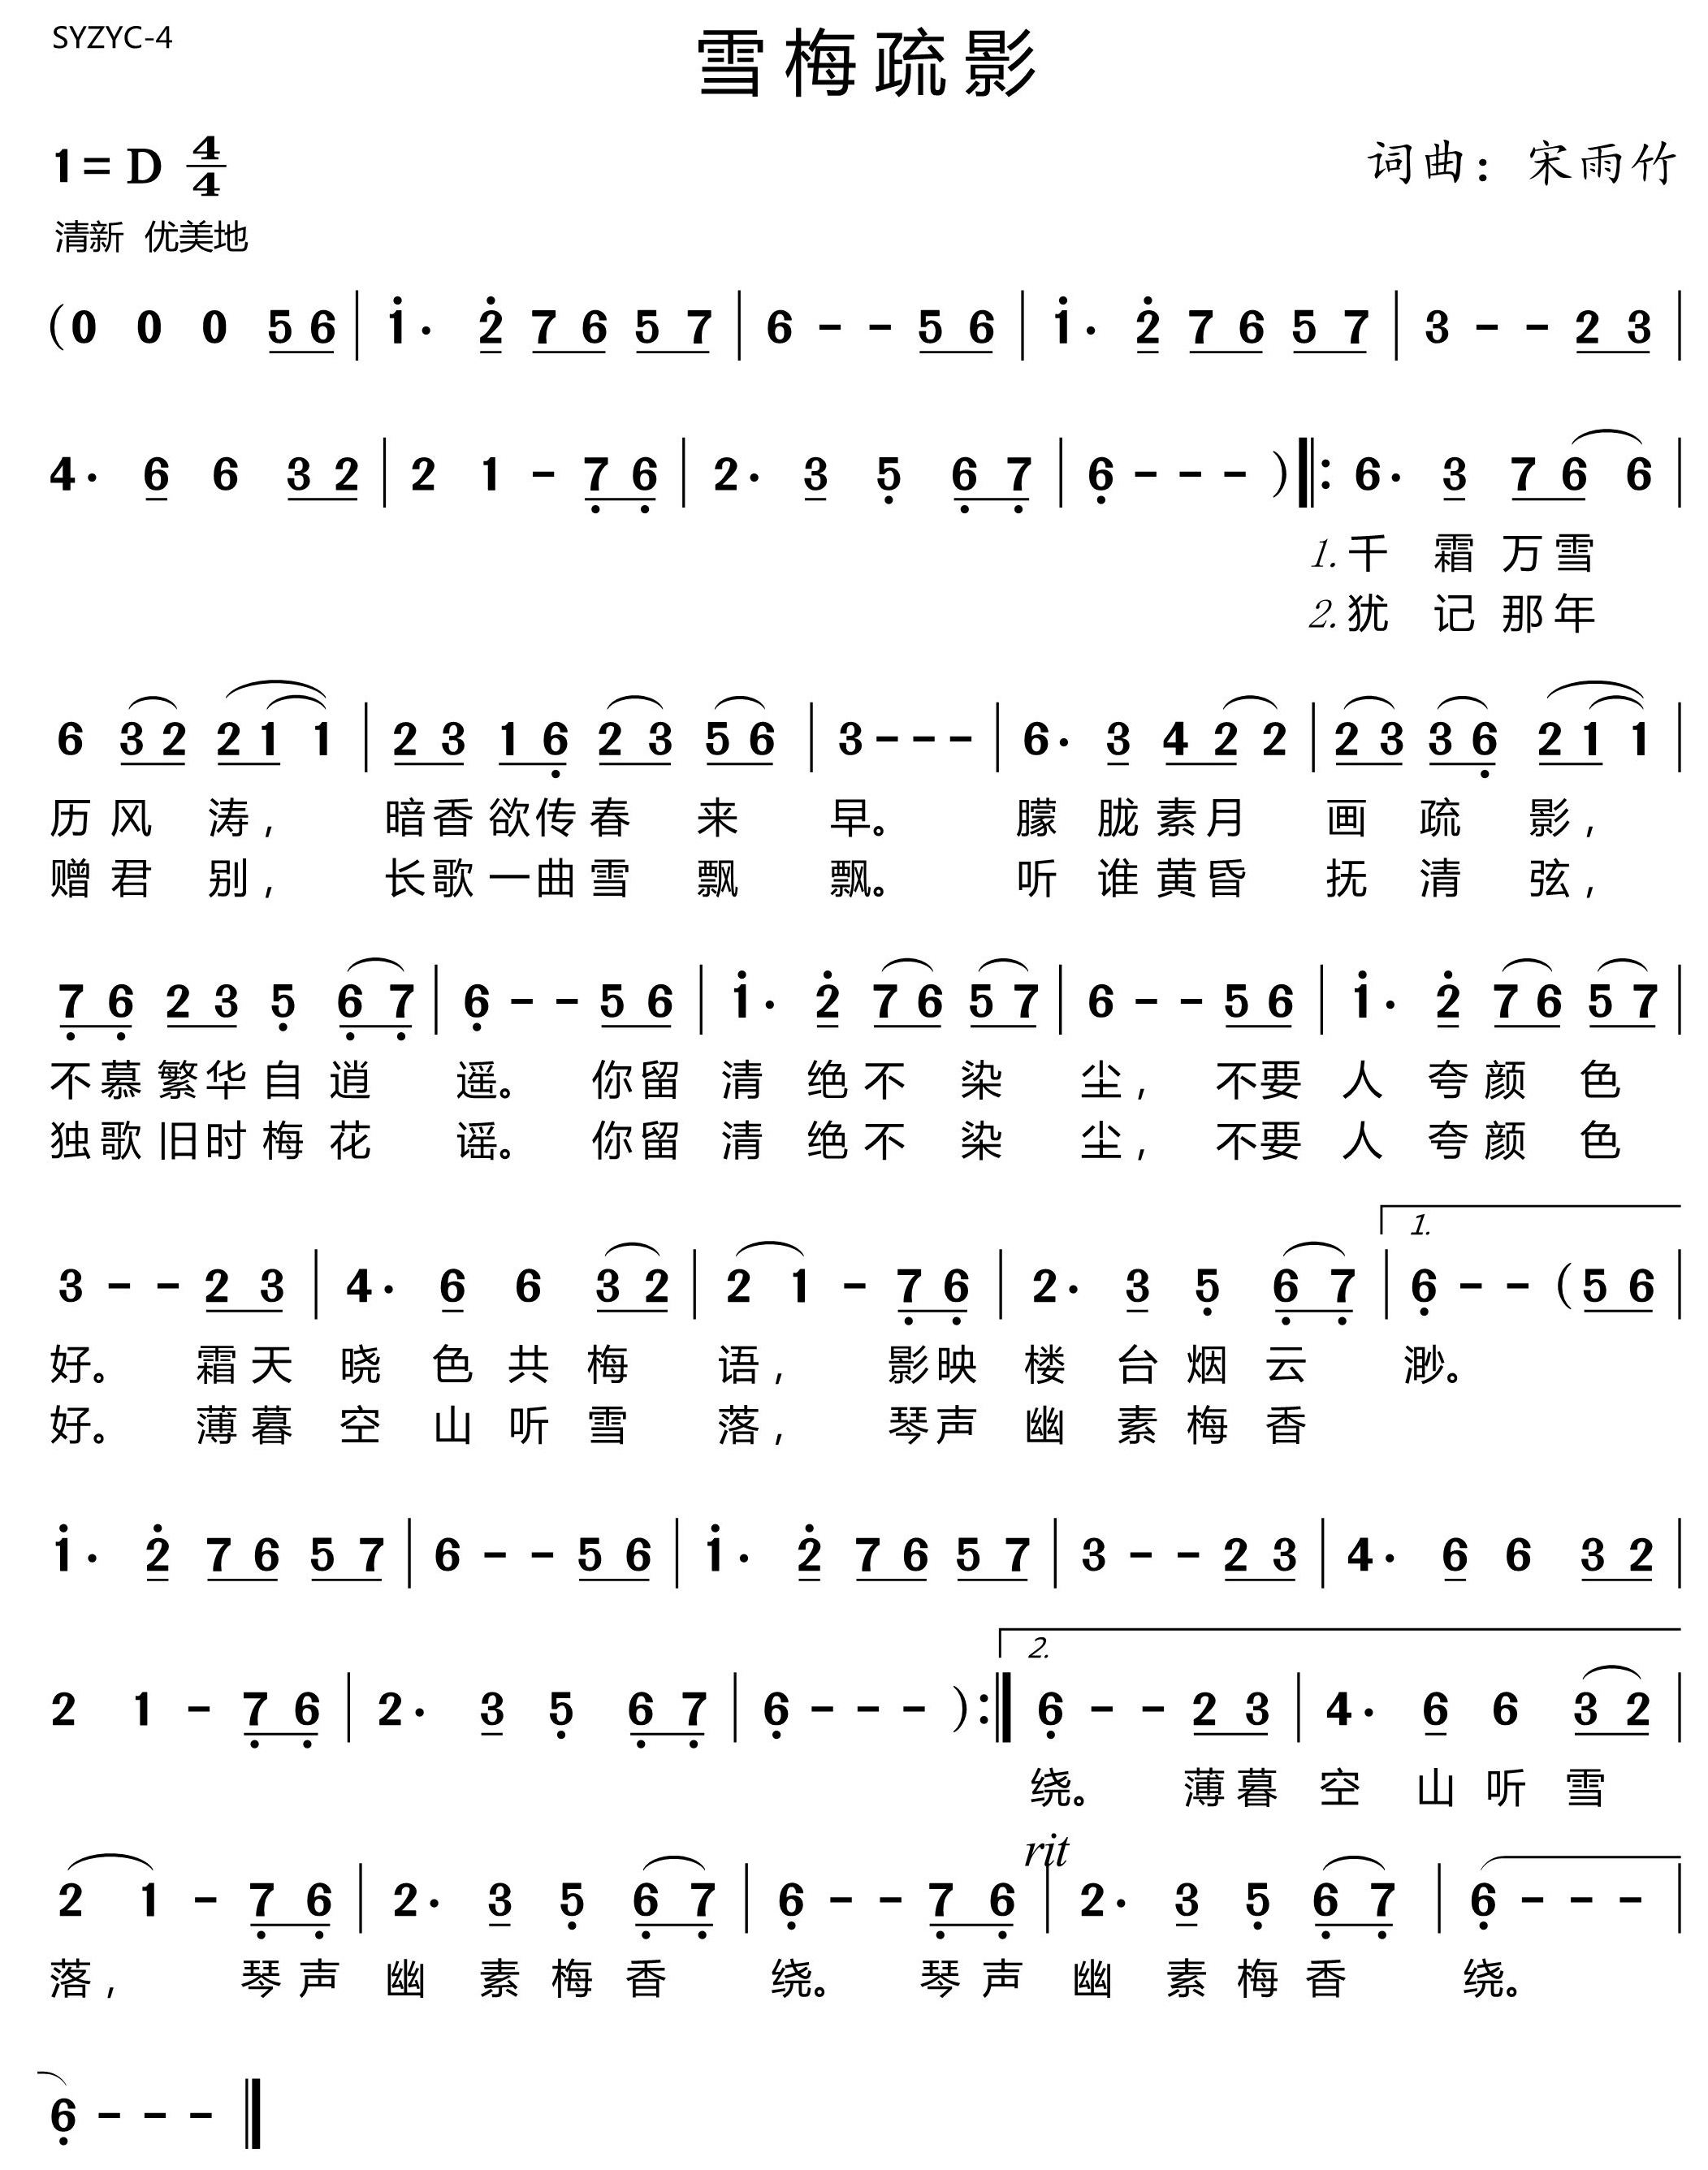
\includegraphics[width=0.9\textwidth]{dongxiao/20200725-雪梅疏影}
\section{静夜思}
    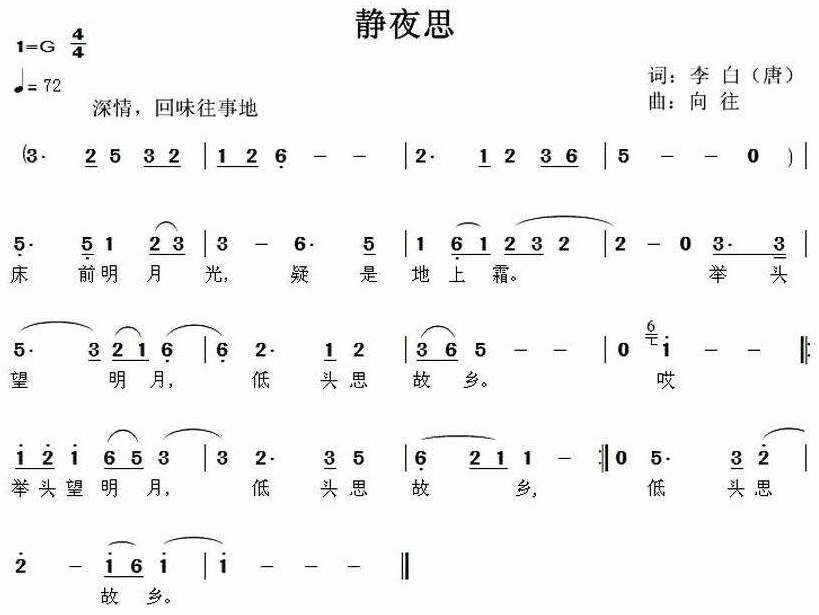
\includegraphics[width=0.9\textwidth]{dongxiao/20200411-静夜思}

\chapter{王维}
\section{山中}
    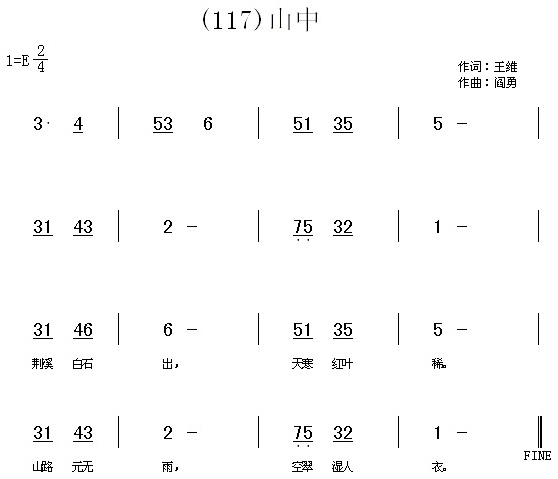
\includegraphics[width=\textwidth]{dongxiao/20200627-王维-山中.jpg}  
\section{\xpinyin*{山居秋暝}}
    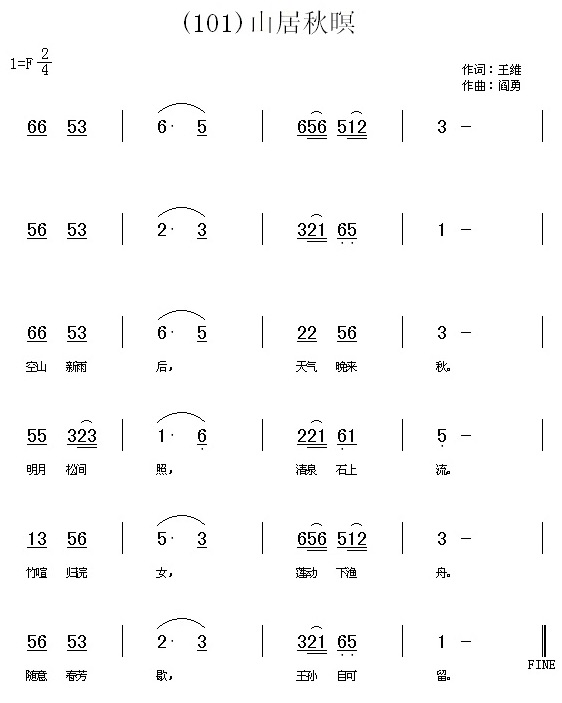
\includegraphics[width=\textwidth]{dongxiao/20200627-王维-山居秋暝.jpg} 
\section{辛夷坞}
    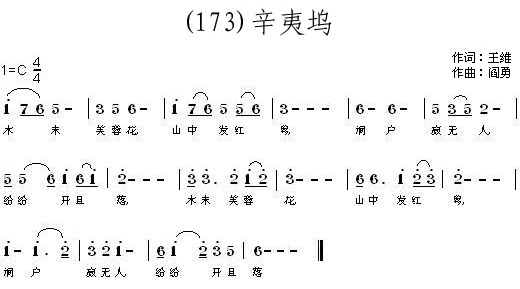
\includegraphics[width=\textwidth]{dongxiao/20200627-王维-辛夷坞.jpg} 
\section{红豆}
    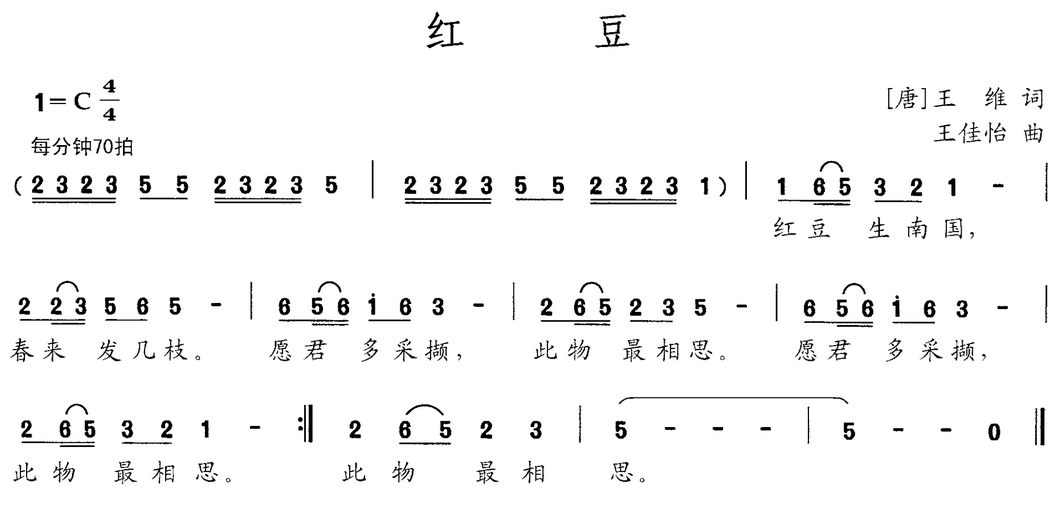
\includegraphics[width=\textwidth]{dongxiao/20200628-王维-红豆} 
\section{鸟鸣涧}
    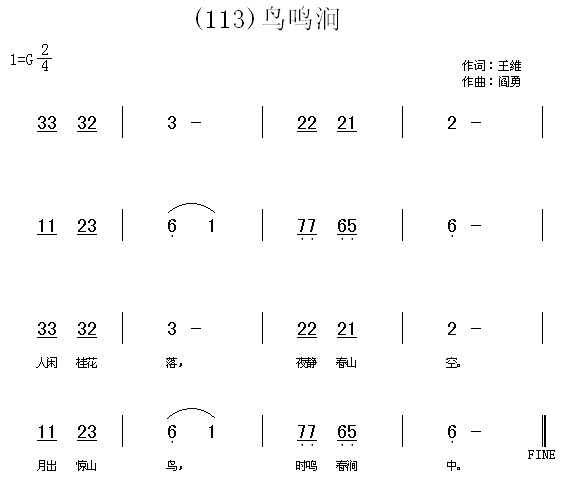
\includegraphics[width=\textwidth]{dongxiao/20200627-王维-鸟鸣涧}

\chapter{苏轼}
\section{黄州定慧院寓居作}
    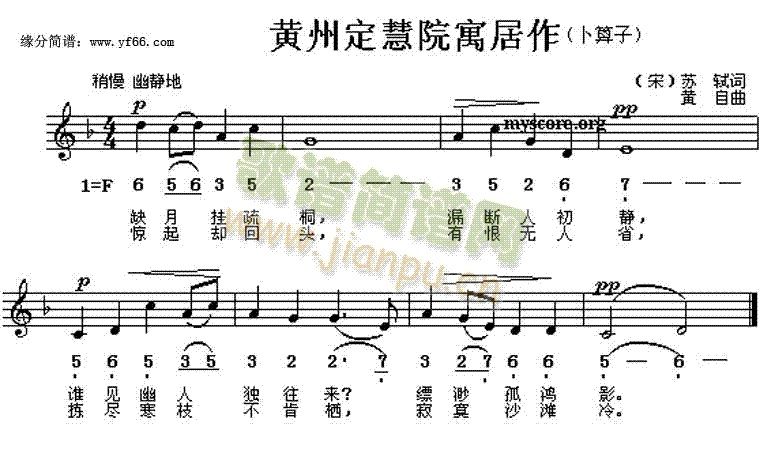
\includegraphics[width=\textwidth]{dongxiao/20200627-苏轼-黄州定慧院寓居作.jpg} 
\section{定风波}
    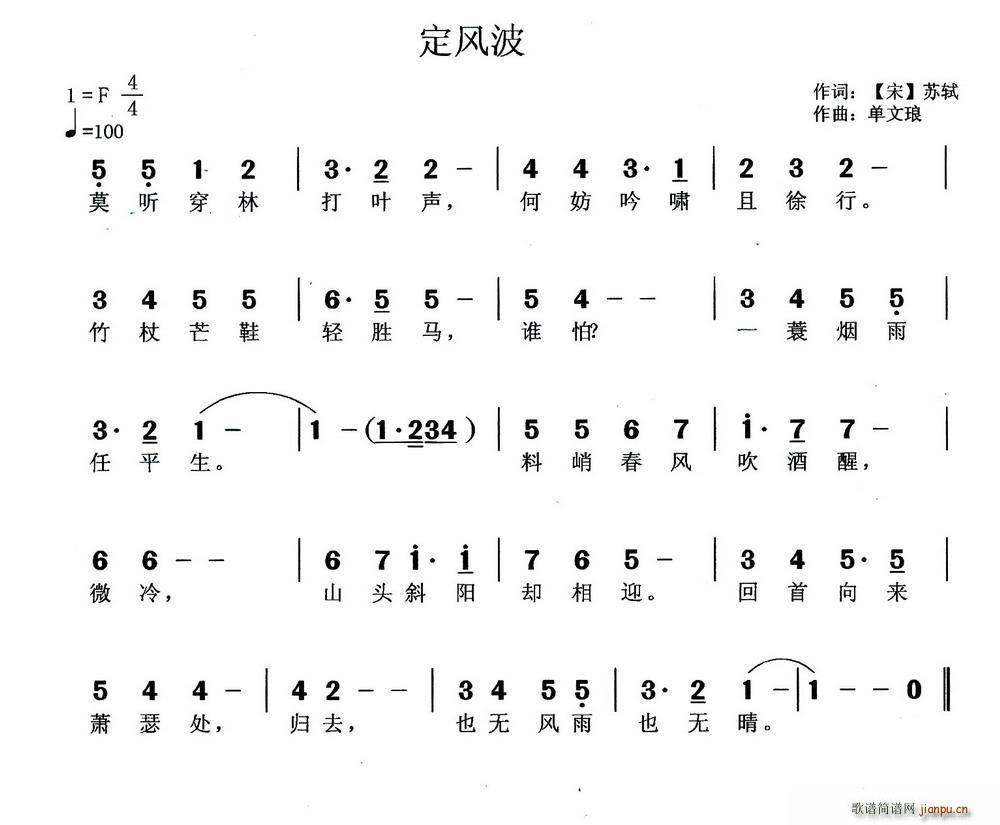
\includegraphics[width=\textwidth]{dongxiao/20200411-定风波.jpg}
\section{蝶恋花-春景}
    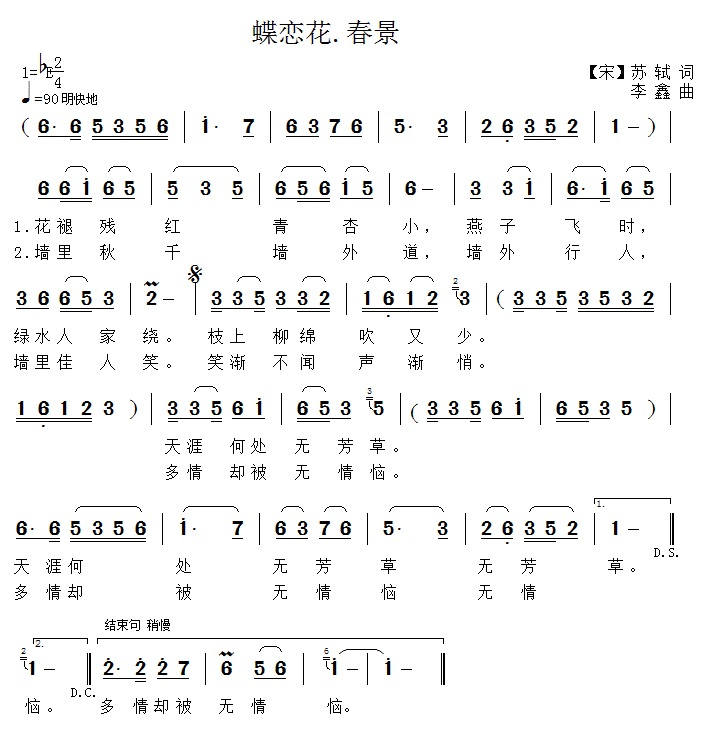
\includegraphics[width=\textwidth]{dongxiao/20200411-蝶恋花-春景.jpg}
\section{六月二十七日望湖楼醉书}
    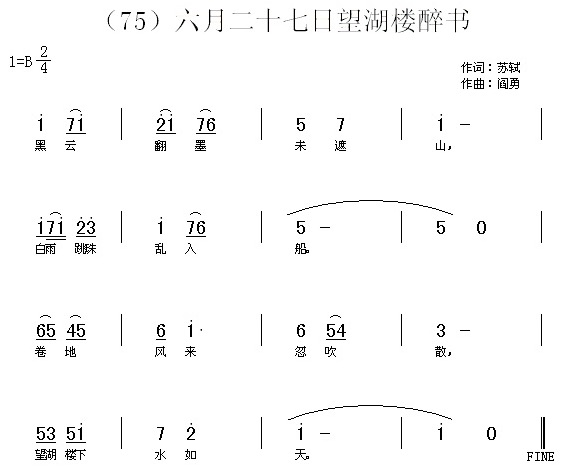
\includegraphics[width=\textwidth]{dongxiao/20200627-苏轼-六月二十七日望湖楼醉书.jpg} 
\section{江城子}
    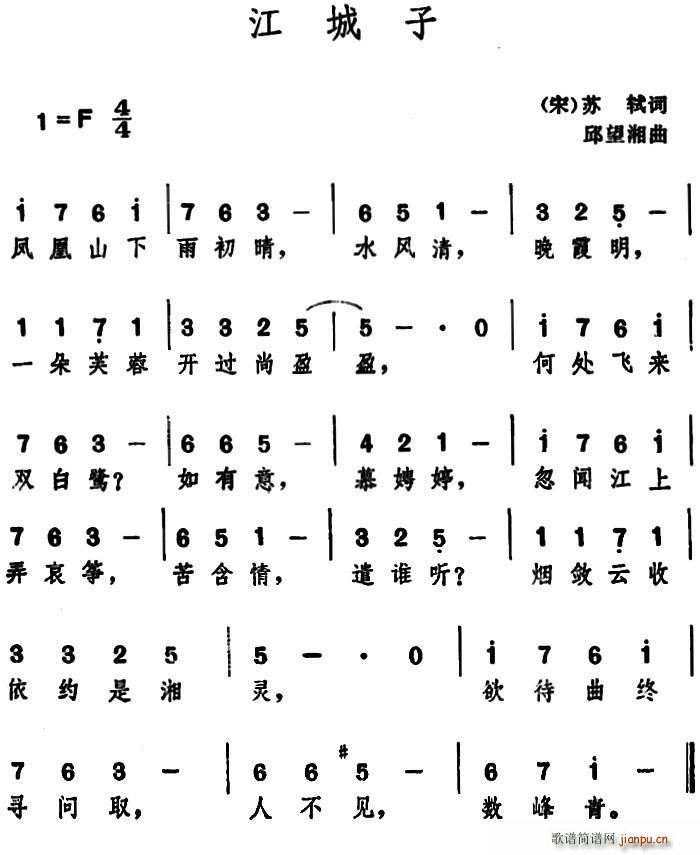
\includegraphics[width=\textwidth]{dongxiao/20200627-苏轼-江城子.jpg} 
\section{花影}
    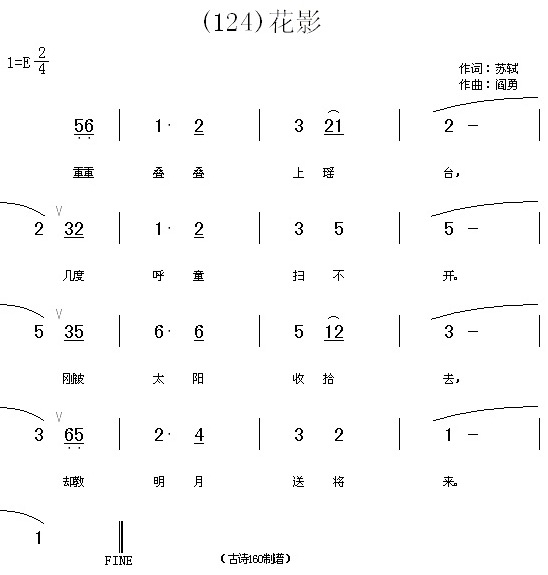
\includegraphics[width=\textwidth]{dongxiao/20200627-苏轼-花影.jpg} 
\section{饮湖上初晴后雨}
    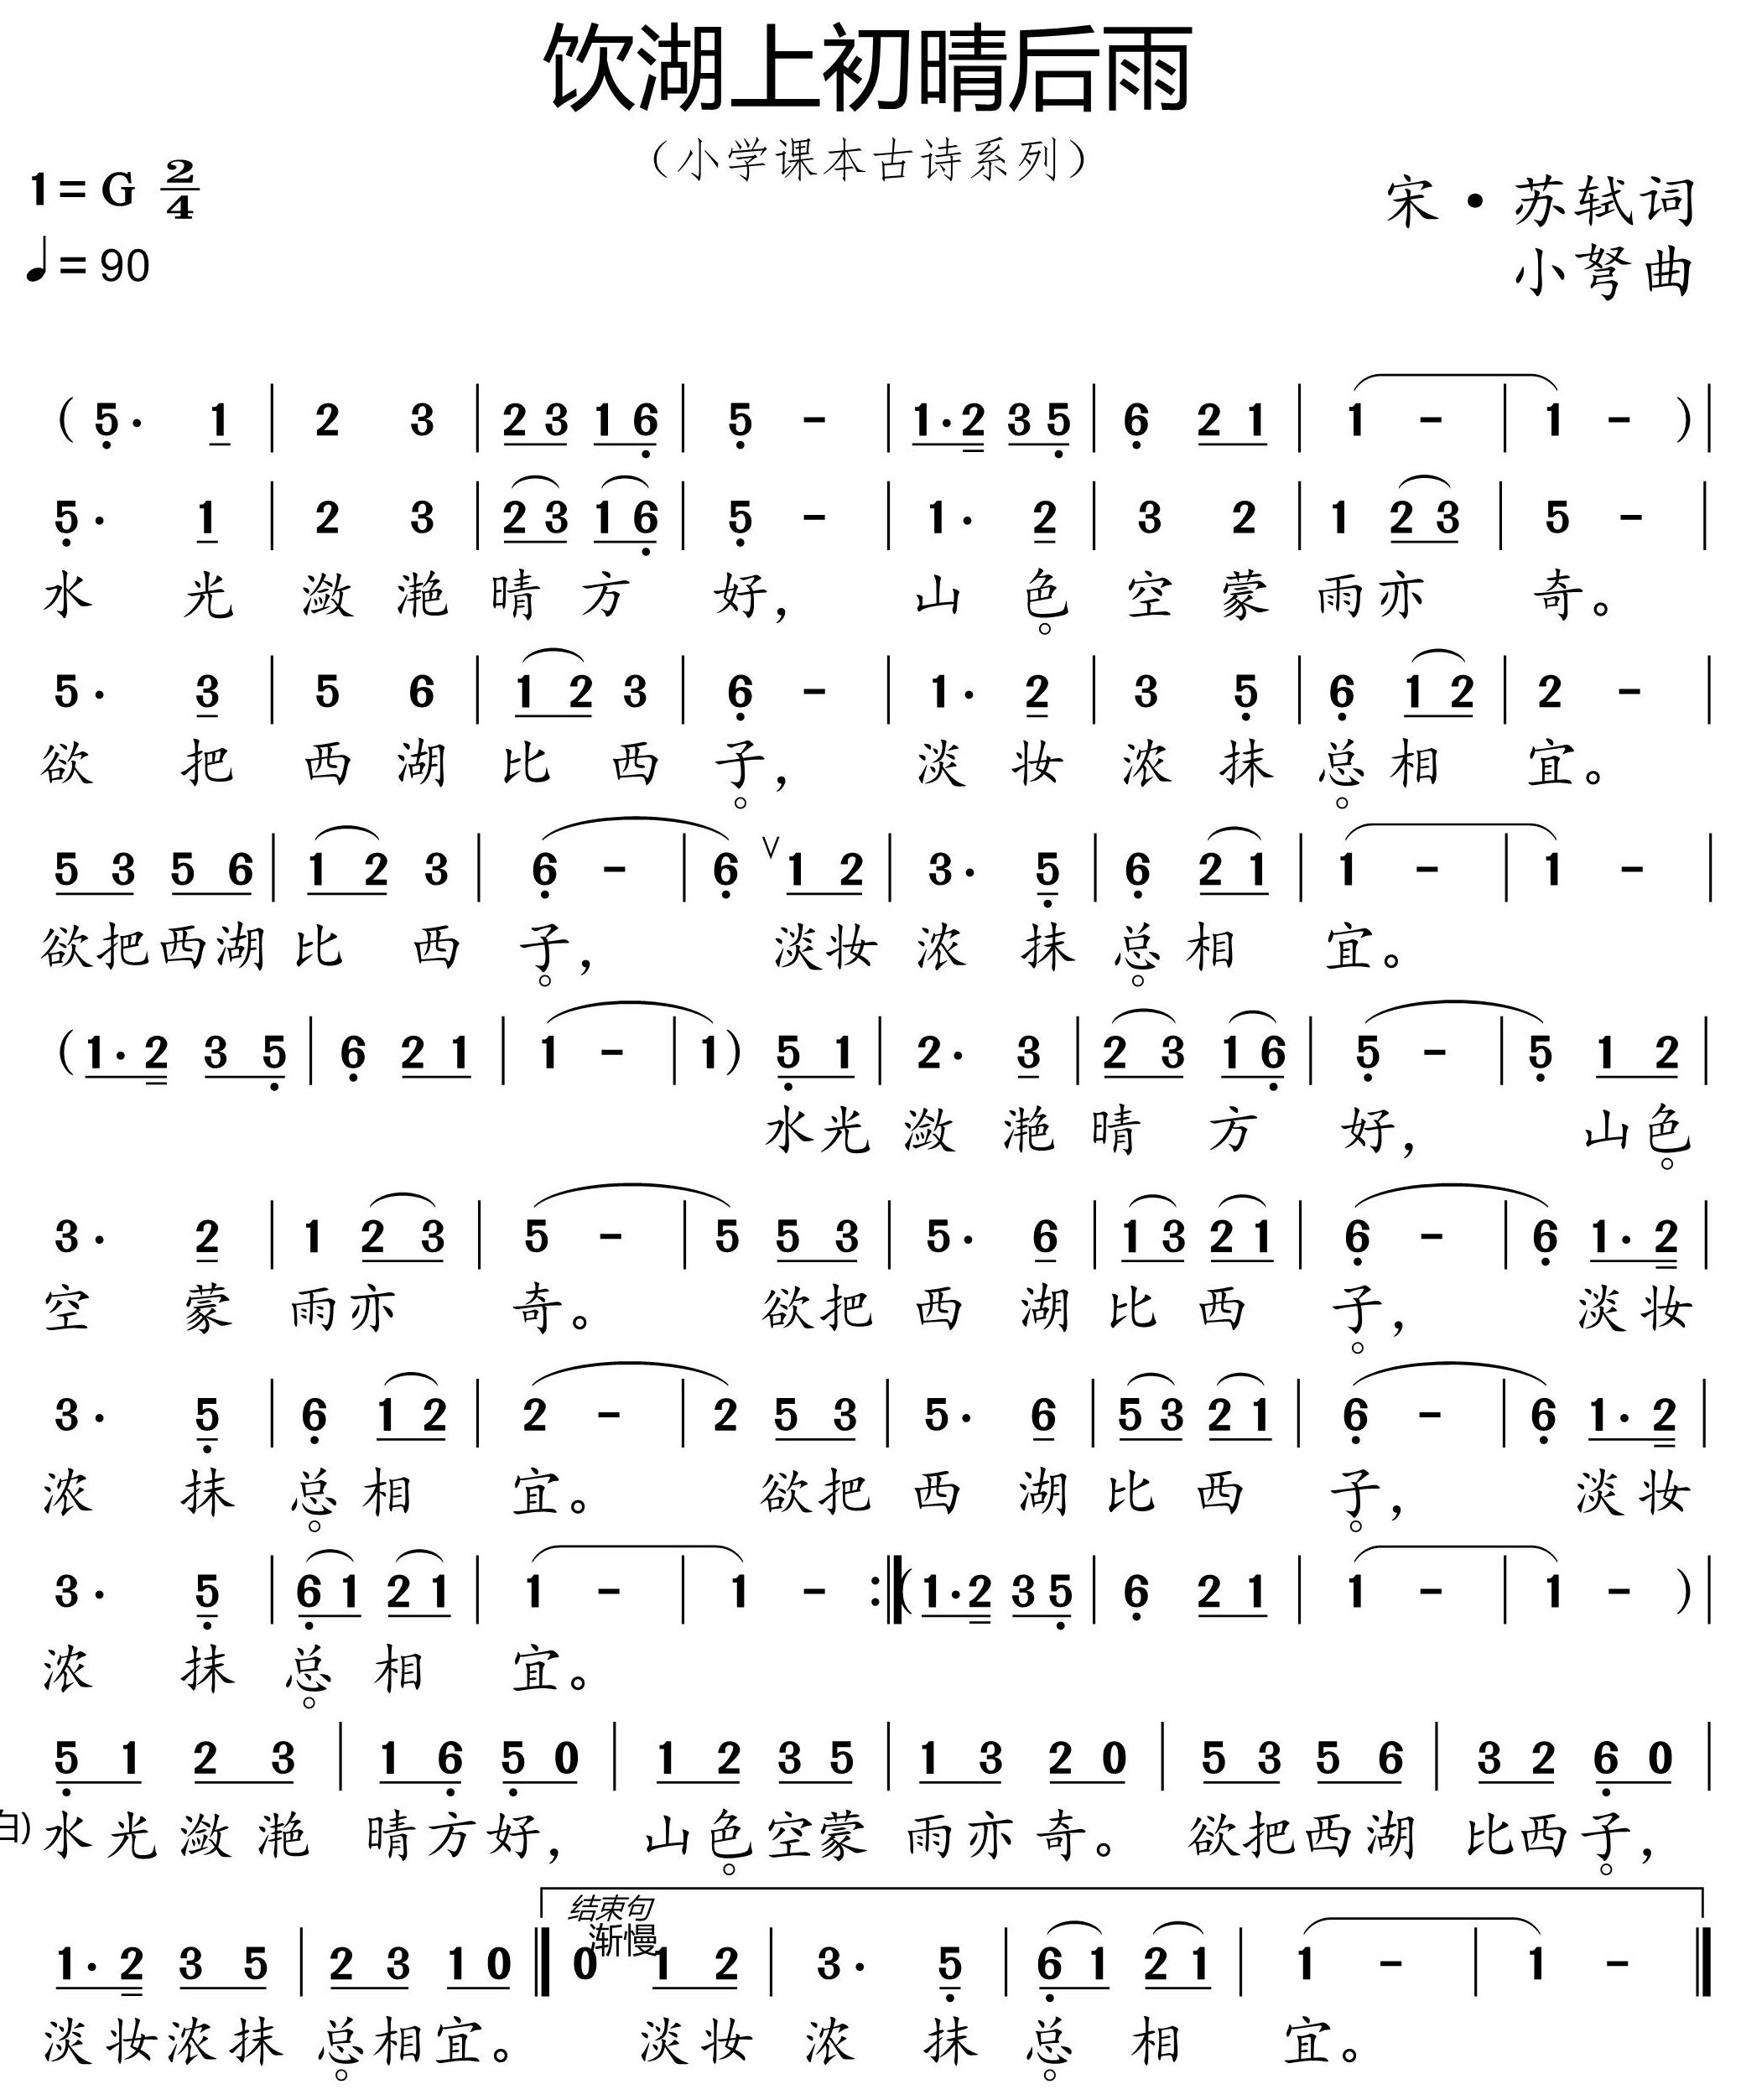
\includegraphics[width=\textwidth]{dongxiao/20200627-苏轼-饮湖上初晴后雨.jpg} 
\section{明月几时有}
    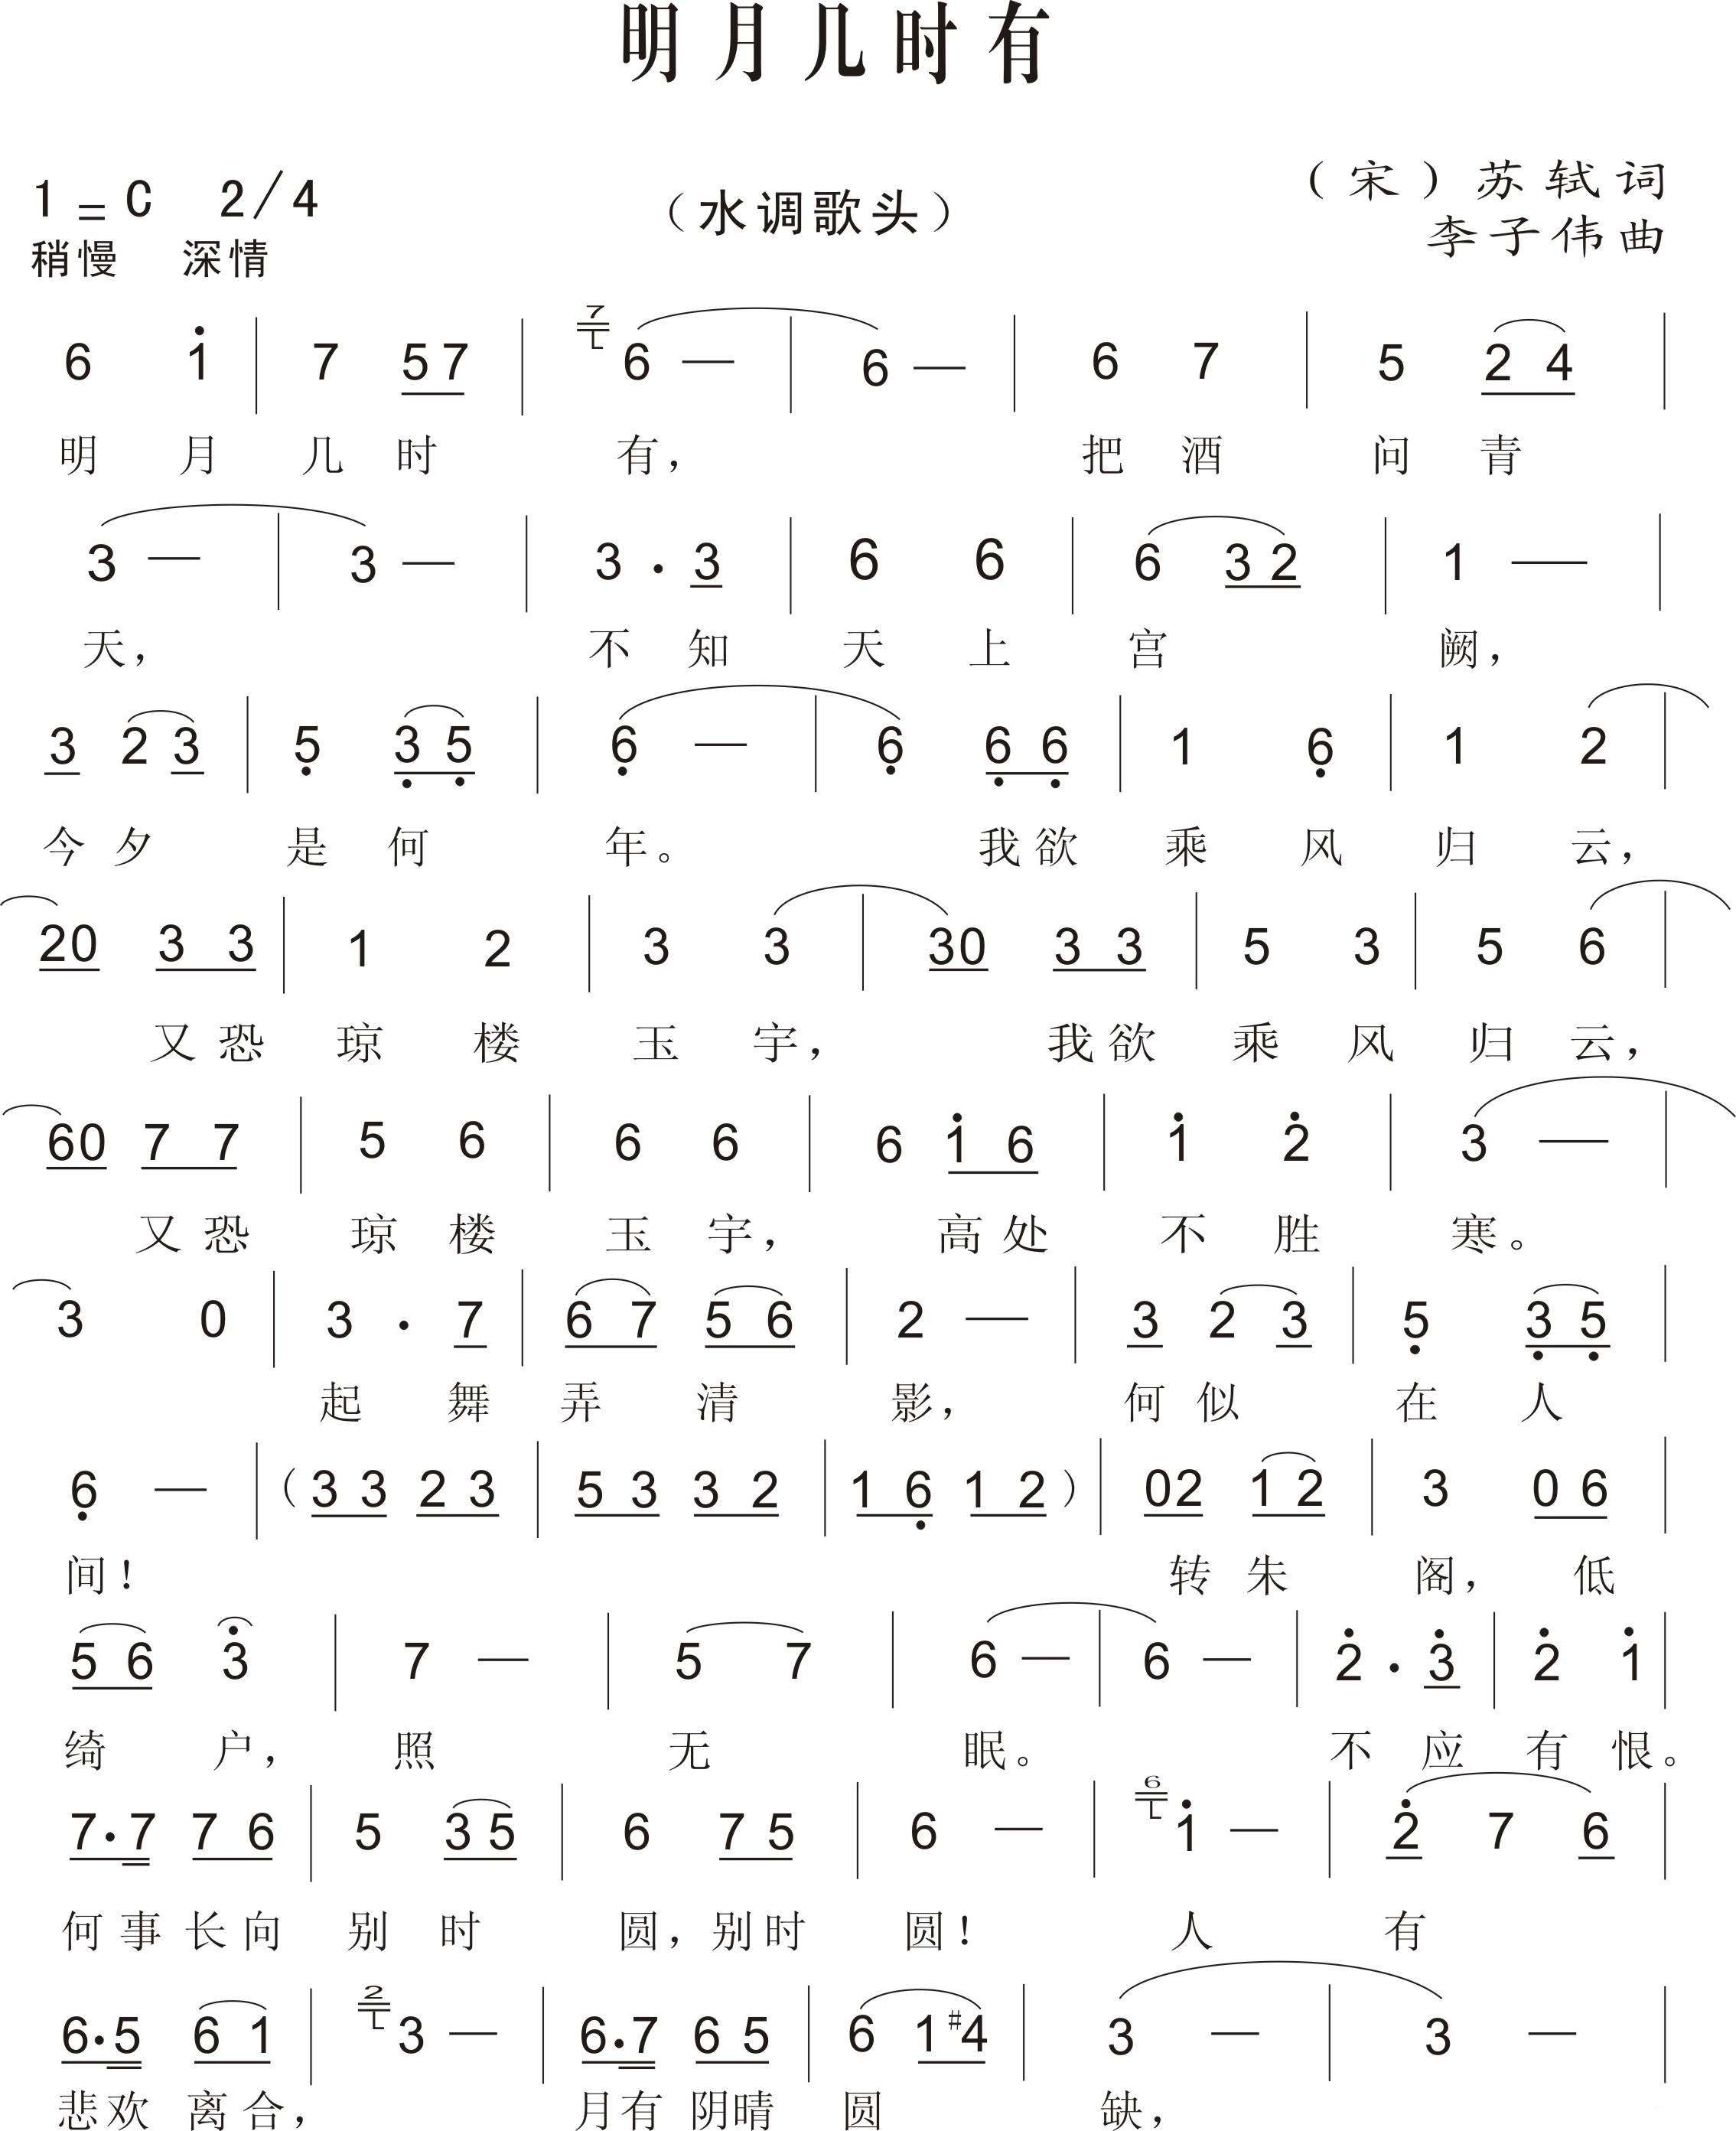
\includegraphics[width=\textwidth]{dongxiao/20200411-明月几时有.jpg}
\section{十年生死两茫茫}
    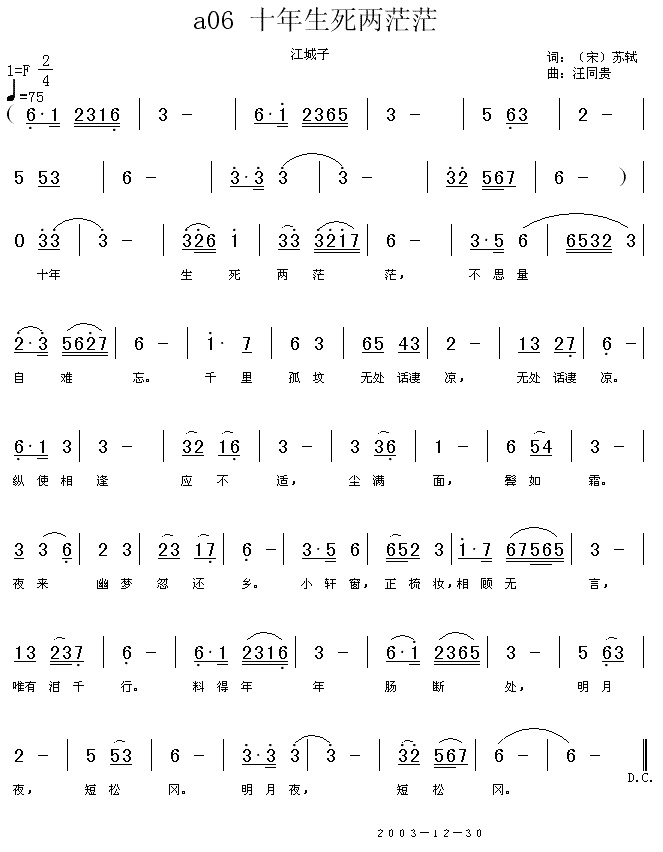
\includegraphics[width=\textwidth]{dongxiao/20200627-苏轼-十年生死两茫茫.jpg} 
\section{念奴娇赤壁怀古}
    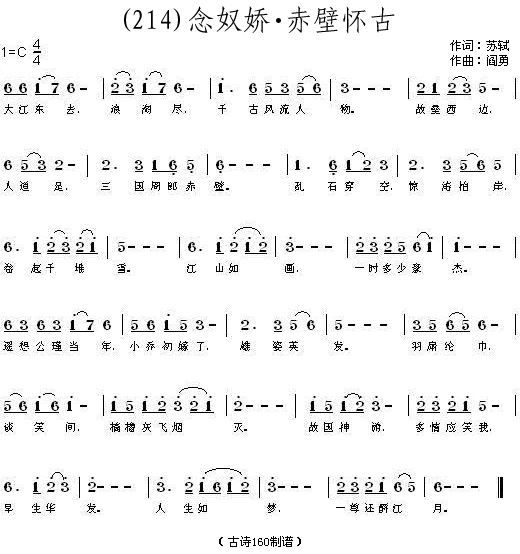
\includegraphics[width=\textwidth]{dongxiao/20200801-苏轼-念奴娇赤壁怀古}
\section{花褪残红青杏小}
    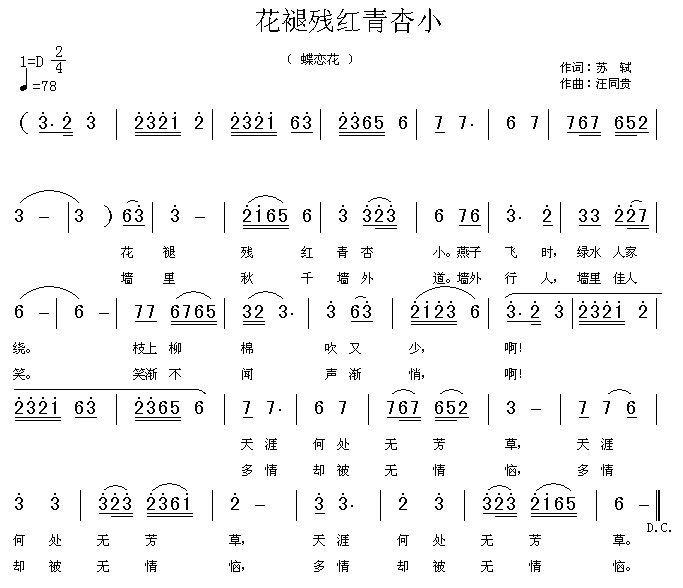
\includegraphics[width=\textwidth]{dongxiao/20200801-苏轼-花褪残红青杏小} 
   
\chapter{李清照}
\section{如梦令}
    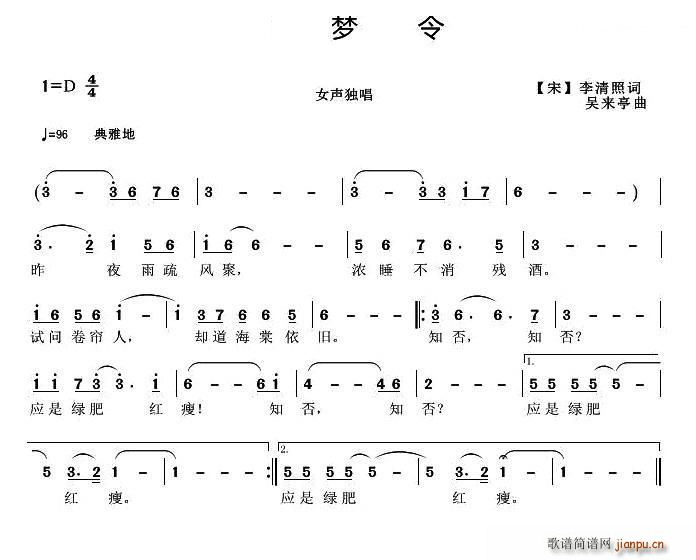
\includegraphics[width=\textwidth]{dongxiao/20200808-如梦令-李清照.jpg}
\section{醉花阴}
    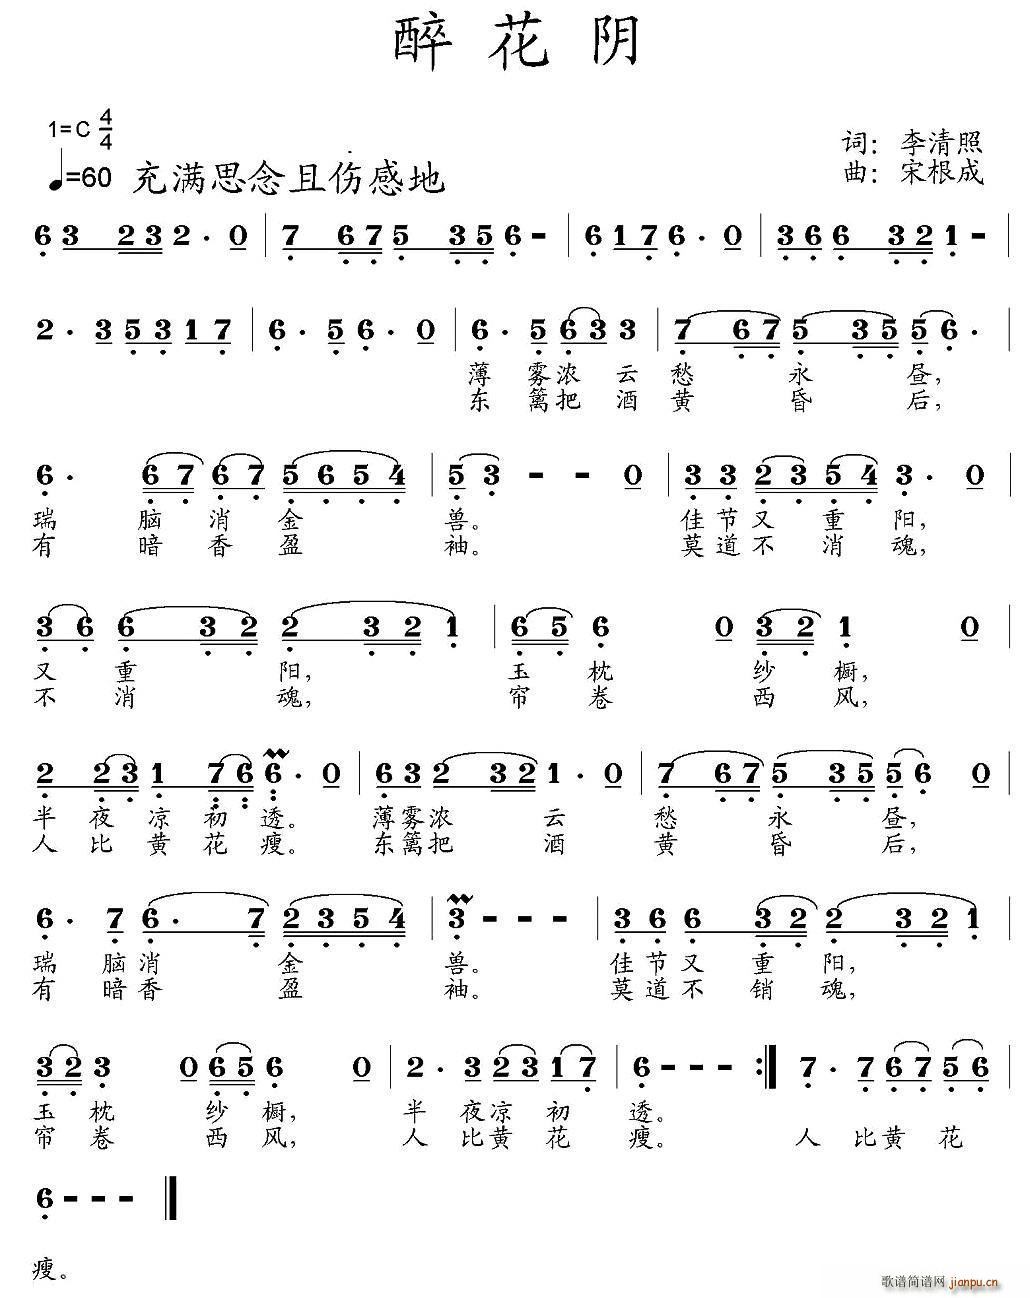
\includegraphics[width=\textwidth]{dongxiao/20200808-醉花阴-李清照.jpg} 
\section{常记溪亭日暮}
    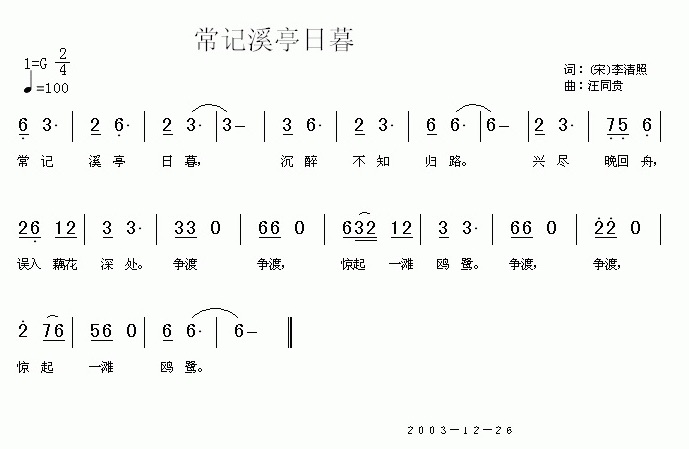
\includegraphics[width=\textwidth]{dongxiao/20200808-常记溪亭日暮-李清照.jpg}
\section{昨夜雨疏风骤}
    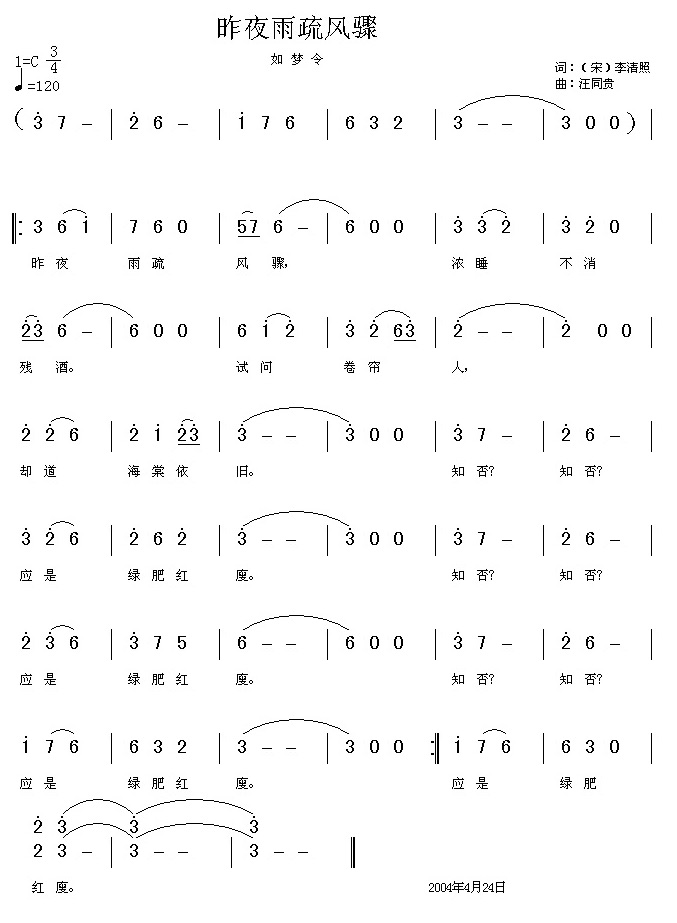
\includegraphics[width=\textwidth]{dongxiao/20200808-昨夜雨疏风骤-李清照.jpg}    
   
\chapter{杜甫}
\section{忆昔}
    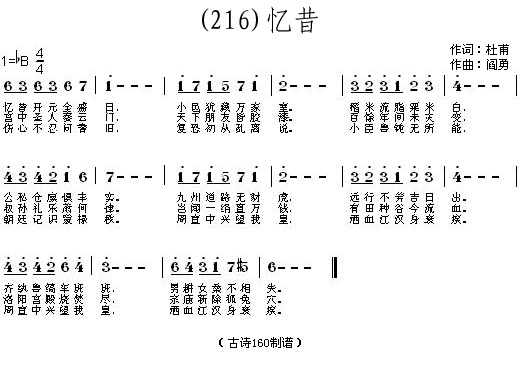
\includegraphics[width=\textwidth]{dongxiao/20200808-忆昔-杜甫.jpg} 
\section{春夜喜雨}
    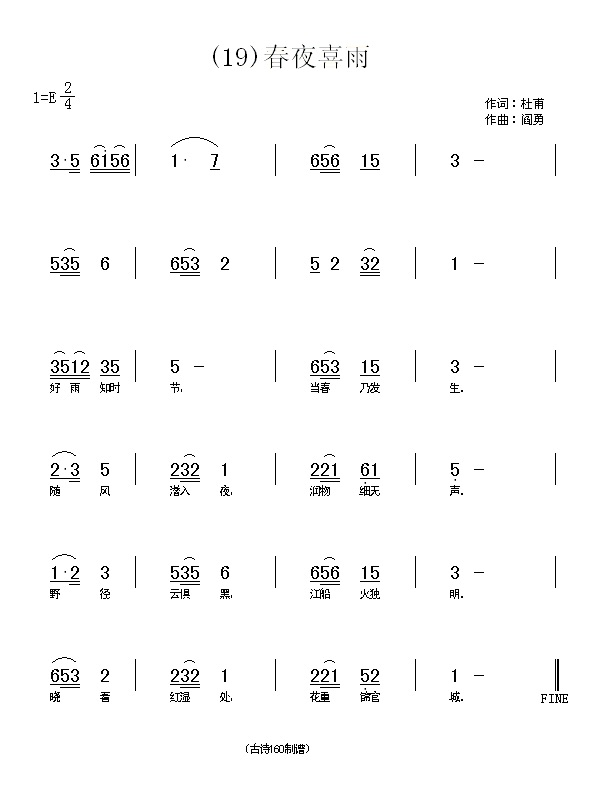
\includegraphics[width=\textwidth]{dongxiao/20200808-春夜喜雨-杜甫.jpg}
\section{春望}
    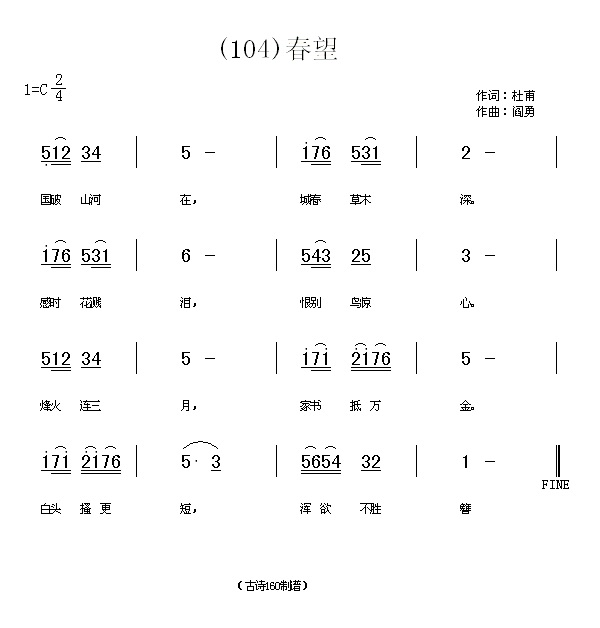
\includegraphics[width=\textwidth]{dongxiao/20200808-春望-杜甫.jpg}
\section{赠花卿}
    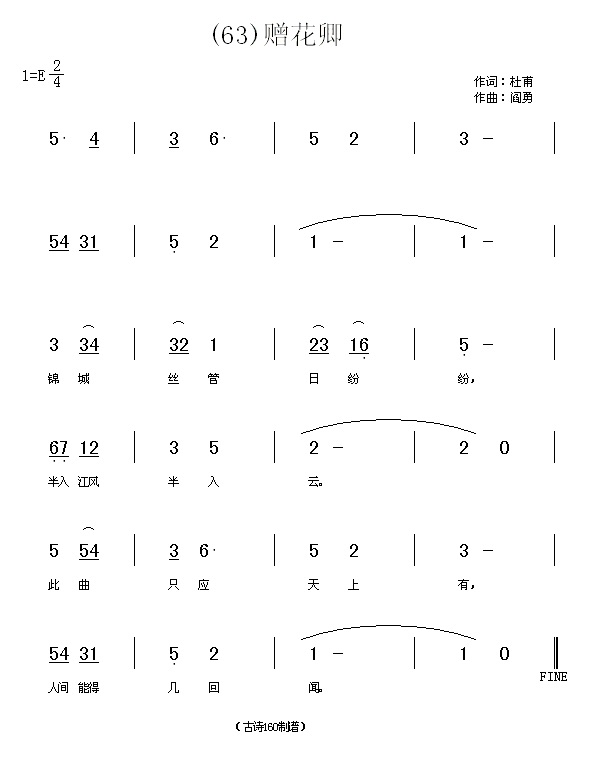
\includegraphics[width=\textwidth]{dongxiao/20200808-赠花卿-杜甫.jpg}    
\section{月夜}
    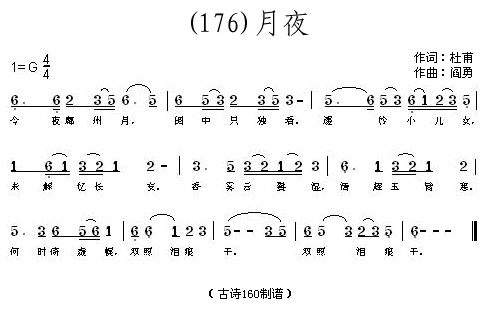
\includegraphics[width=\textwidth]{dongxiao/20200808-月夜-杜甫.jpg}                     
\section{江畔独步寻花}
    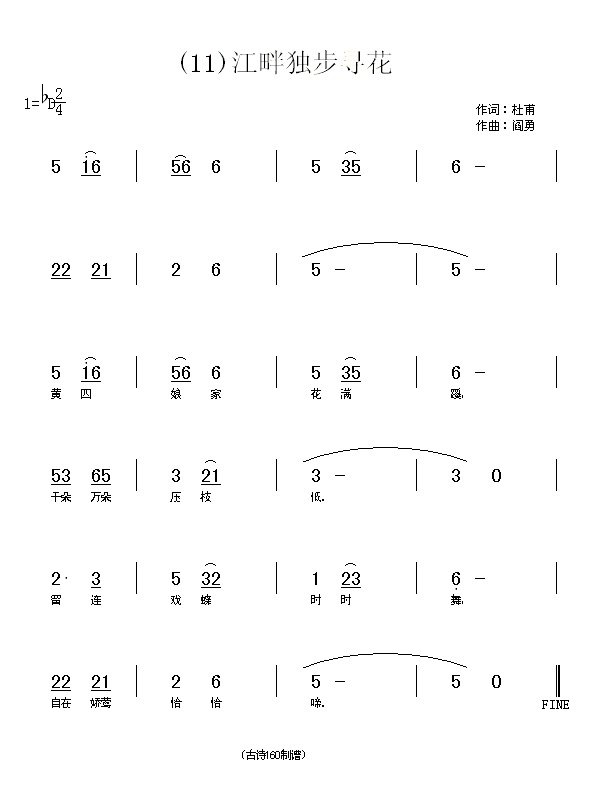
\includegraphics[width=\textwidth]{dongxiao/20200808-江畔独步寻花-杜甫.jpg}   

\chapter{李白}
\section{忆秦娥}
    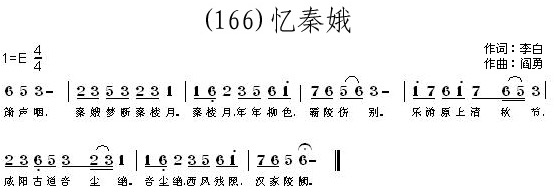
\includegraphics[width=\textwidth]{dongxiao/20200808-忆秦娥-李白.jpg} 
\section{怨情}
    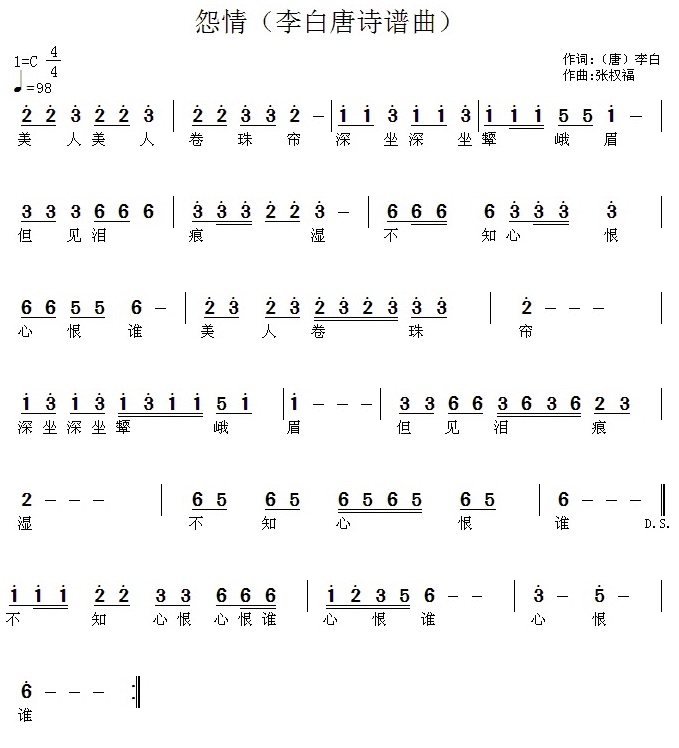
\includegraphics[width=\textwidth]{dongxiao/20200808-怨情-李白.jpg}
\section{春思}
    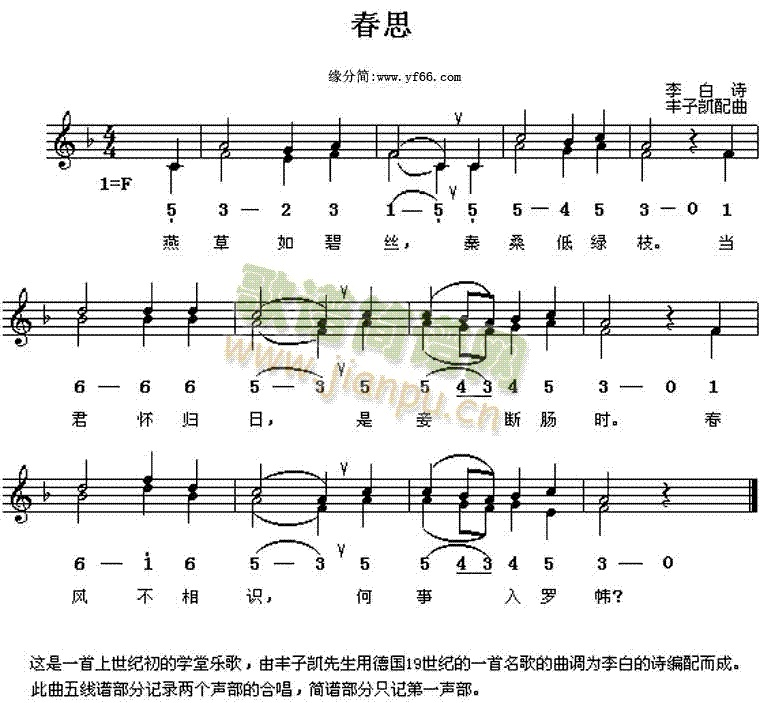
\includegraphics[width=\textwidth]{dongxiao/20200808-春思-李白.jpg}
\section{古朗月行}
    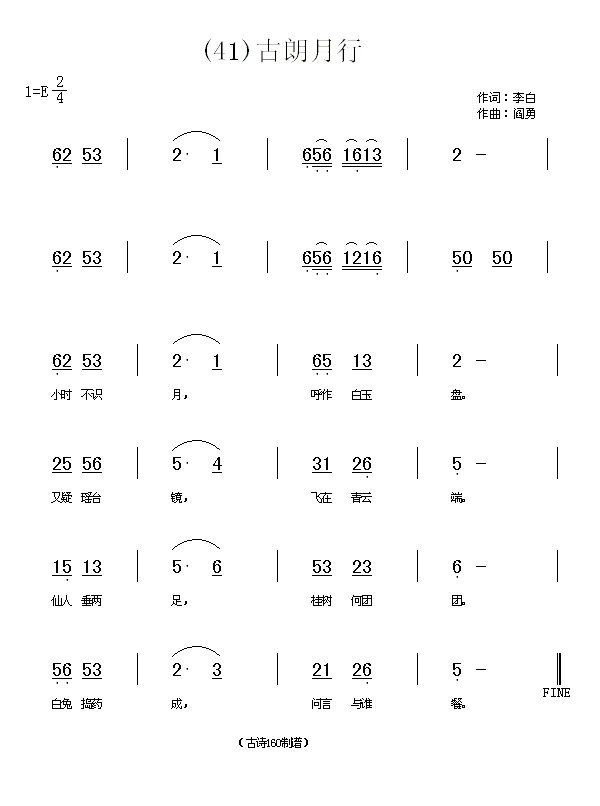
\includegraphics[width=\textwidth]{dongxiao/20200808-古朗月行-李白.jpg}    
\section{月下独酌}
    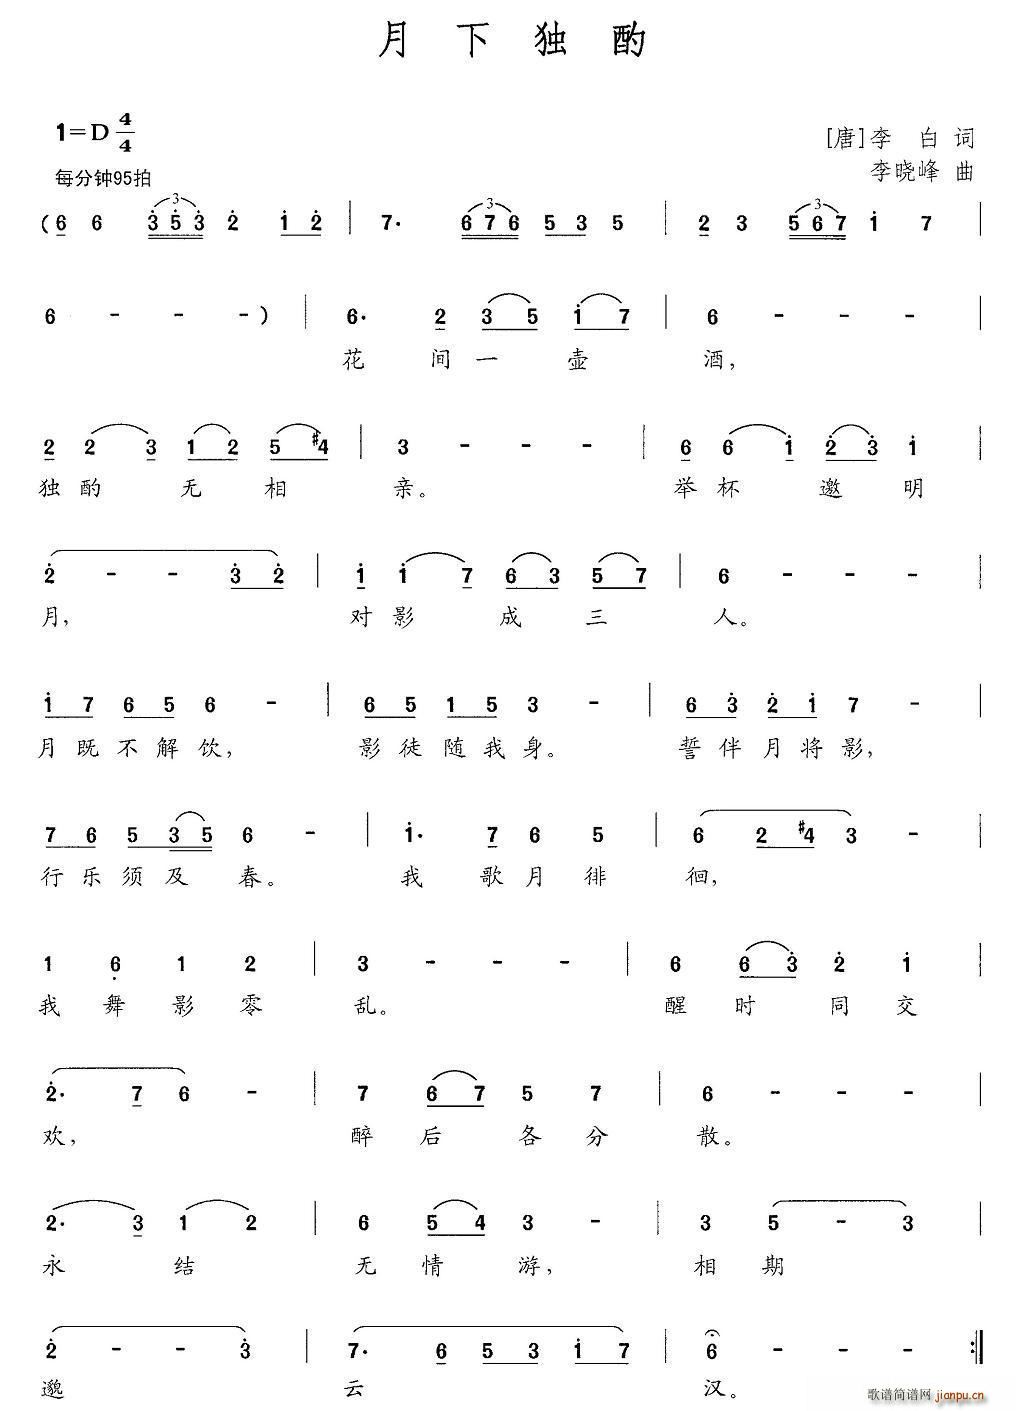
\includegraphics[width=0.95\textwidth]{dongxiao/20200808-月下独酌-李白.jpg} 
\section{秋浦歌}
    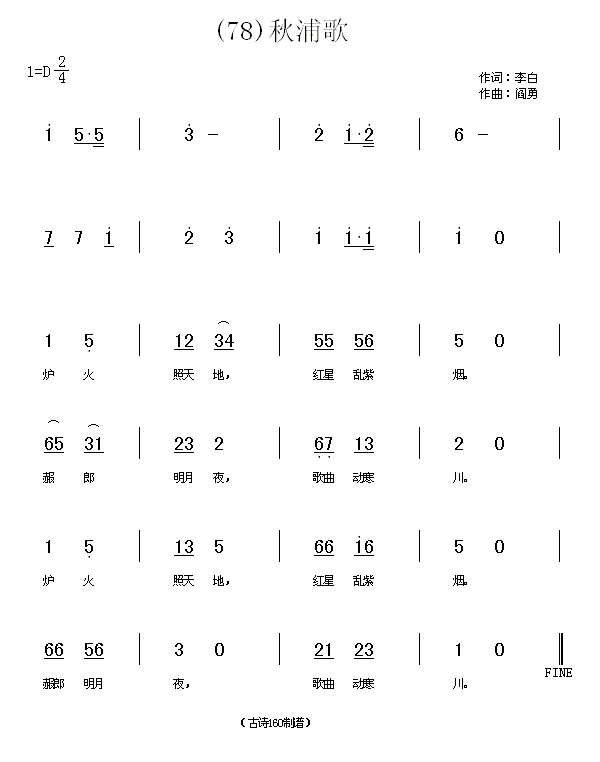
\includegraphics[width=\textwidth]{dongxiao/20200808-秋浦歌-李白.jpg}
\section{独坐敬亭山}
    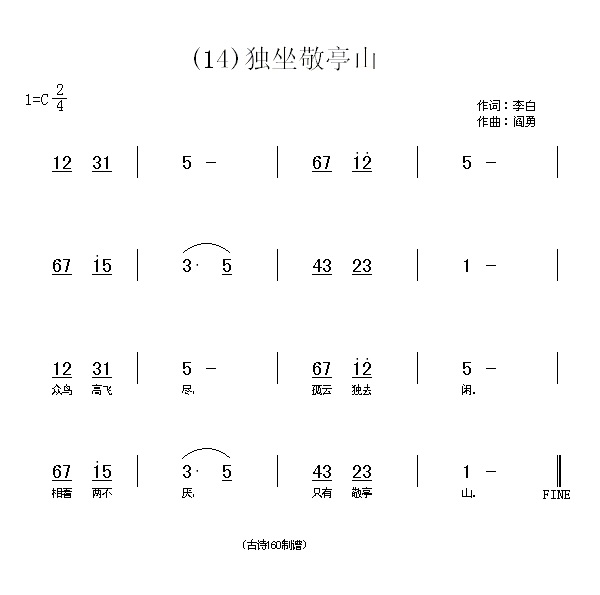
\includegraphics[width=\textwidth]{dongxiao/20200808-独坐敬亭山-李白.jpg}
\section{望庐山瀑布}
    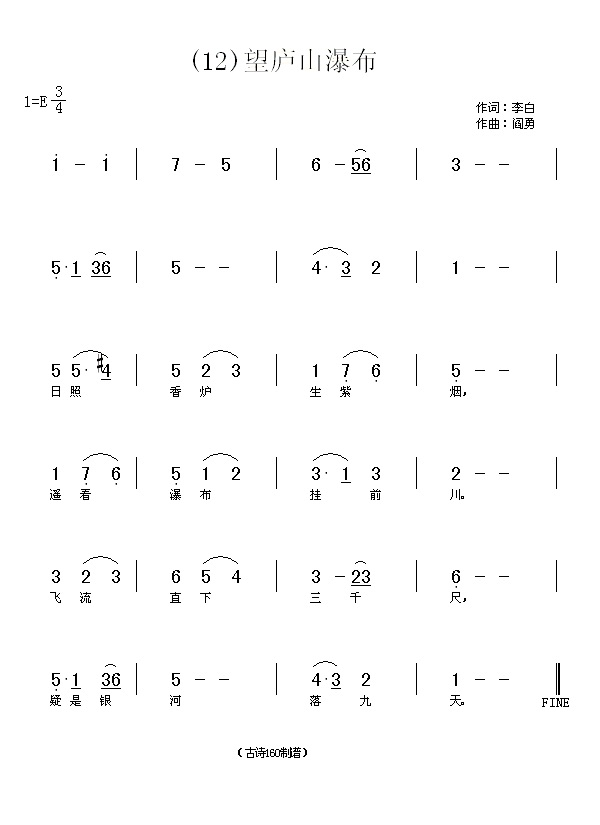
\includegraphics[width=\textwidth]{dongxiao/20200808-望庐山瀑布-李白.jpg}
\section{美人怨}
    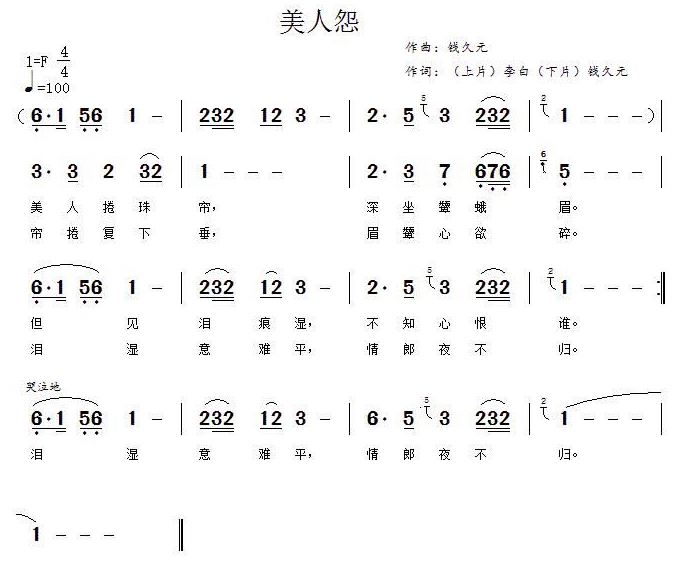
\includegraphics[width=\textwidth]{dongxiao/20200808-美人怨-李白.jpg}
\section{菩萨蛮}
    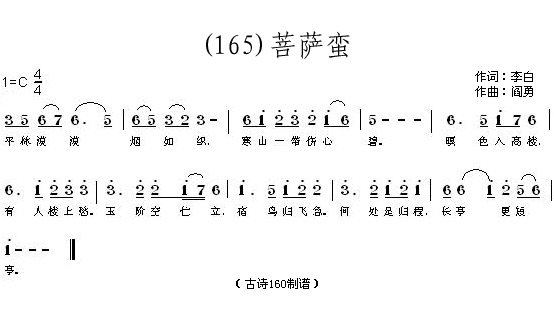
\includegraphics[width=\textwidth]{dongxiao/20200808-菩萨蛮-李白.jpg}

\chapter{曹操}
\section{忆秦娥}
    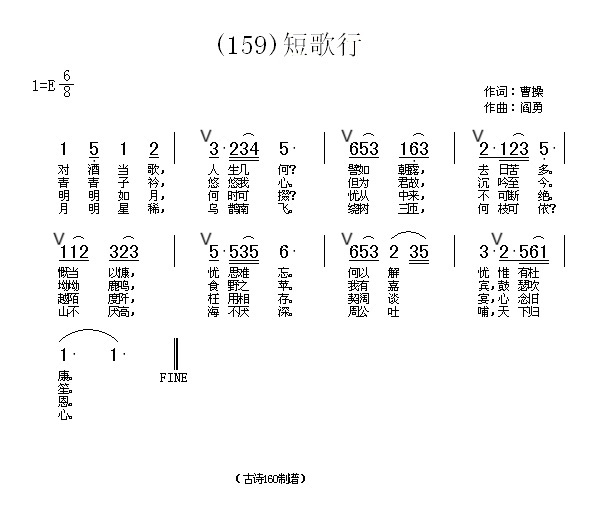
\includegraphics[width=\textwidth]{dongxiao/20200808-短歌行-曹操.jpg} 
\section{怨情}
    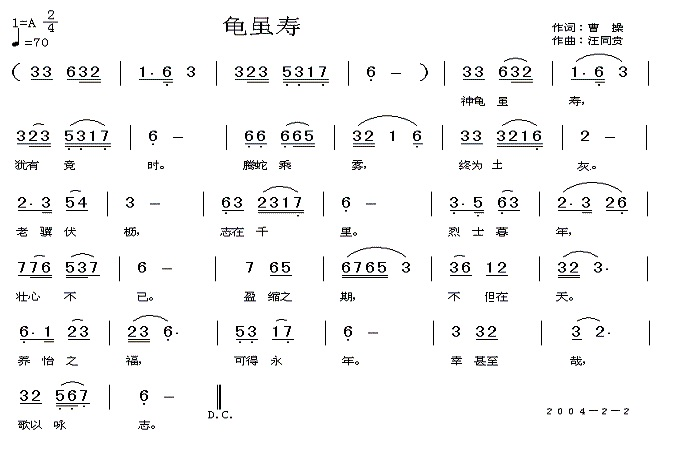
\includegraphics[width=\textwidth]{dongxiao/20200808-神龟虽寿-曹操.jpg}
\section{春思}
    \includegraphics[width=0.95\textwidth]{dongxiao/20200808-观沧海-曹操.jpg}                             
                           
                          
         
\chapter{陆游}
\section{示儿}
    \includegraphics[width=\textwidth]{dongxiao/20200808-示儿-陆游.jpg} 
\section{红酥手}
    \includegraphics[width=\textwidth]{dongxiao/20200808-红酥手-陆游.jpg}
\section{钗头凤}
    \includegraphics[width=0.7\textwidth]{dongxiao/20200808-钗头凤-陆游.jpg}                             
\section{题临安邸}
    \includegraphics[width=\textwidth]{dongxiao/20200808-题临安邸-陆游.jpg}                             
 
\chapter{古诗}
\section{乞巧(唐,林杰)}
    \includegraphics[width=\textwidth]{dongxiao/20200627-古诗-乞巧.jpg}     
\section{咏柳(唐,贺知章)}
    \includegraphics[width=0.9\textwidth]{dongxiao/20200627-古诗-咏柳.jpg}   
\section{夜书所见(宋,叶绍翁)}
    \includegraphics[width=0.8\textwidth]{dongxiao/20200627-古诗-夜书所见.jpg}   
\section{春日(宋,朱熹)}
    \includegraphics[width=0.8\textwidth]{dongxiao/20200627-古诗-春日.jpg}   
\section{望洞庭(唐,刘禹锡)}
    \includegraphics[width=\textwidth]{dongxiao/20200627-古诗-望洞庭.jpg}   
\section{绝句(唐,杜甫)}
    \includegraphics[width=0.8\textwidth]{dongxiao/20200627-古诗-杜甫-绝句.jpg}   
\section{秋思(唐,张籍)}
    \includegraphics[width=\textwidth]{dongxiao/20200627-古诗-秋思.jpg}   
\section{草(唐,白居易)}
    \includegraphics[width=0.9\textwidth]{dongxiao/20200627-古诗-草.jpg}   
\section{赠汪伦(唐,李白)}
    \includegraphics[width=0.9\textwidth]{dongxiao/20200627-古诗-赠汪伦.jpg}   
\section{已亥杂诗(清,龚自珍)}
    \includegraphics[width=\textwidth]{dongxiao/20200627-古诗-龚自珍-已亥杂诗.jpg}   
\section{枫桥夜泊}
    \includegraphics[width=\textwidth]{dongxiao/20200808-枫桥夜泊-昆曲.jpg}   
\section{枫桥夜泊2}
    \includegraphics[width=\textwidth]{dongxiao/20200808-枫桥夜泊-张继.jpg}  
                            
  
\chapter{日本歌譜}
\section{樱花}
	\includegraphics[width=\textwidth]{dongxiao/日本-樱花.jpg}  
\section{风的大地}
	\includegraphics[width=\textwidth]{dongxiao/20200628-日本-风的大地}  
\section{黎明之歌}
	\includegraphics[width=\textwidth]{dongxiao/20200628-日本-黎明之歌}  
	
\chapter{好妹妹乐队}
\section{南来的風}
    \includegraphics[width=\textwidth]{dongxiao/20200516-好妹妹-南来的风.jpg} 
    
\chapter{雜錄}
\section{长城谣}
    \includegraphics[width=\textwidth]{dongxiao/20200711-长城谣.jpg}
\section{有所思}
    \includegraphics[width=\textwidth]{dongxiao/20200710-有所思}
\section{西湖春}
    \includegraphics[width=\textwidth]{dongxiao/20200711-西湖春.jpg}
\section{茉莉花}
    \includegraphics[width=\textwidth]{dongxiao/20200711-茉莉花.jpg}
\section{苏武牧羊}
    \includegraphics[width=\textwidth]{dongxiao/20200711-苏武牧羊.jpeg}
\section{关山月}
    \includegraphics[width=\textwidth]{dongxiao/20200411-清平乐-关山月.jpg}
\section{清平乐-春归何处}
    \includegraphics[width=\textwidth]{dongxiao/20200411-清平乐-春归何处.jpg}
\section{清平乐-晏殊词}
    \includegraphics[width=\textwidth]{dongxiao/20200411-清平乐-晏殊.jpg}
\section{时间都去哪儿了}
    \includegraphics[width=\textwidth]{dongxiao/20200411-时间都去哪儿了.jpg} 
\section{城市很静}
    \includegraphics[width=\textwidth]{dongxiao/20200402-城市很静} 
\section{玉楼春}
    \includegraphics[width=\textwidth]{dongxiao/20200323玉楼春.jpg}
\section{墨香-长安曲}
    \includegraphics[width=0.9\textwidth]{dongxiao/20200323墨香-长安曲.jpg} 
\section{思美人兮}
    \includegraphics[width=\textwidth]{dongxiao/20200402-思美人.jpg}
\section{無羈}
    \includegraphics[width=\textwidth]{dongxiao/20201231-無羈} 
\section{心經}
    \includegraphics[width=\textwidth]{dongxiao/20201231-心经} 
\section{柳林坡}
    \includegraphics[width=\textwidth]{dongxiao/20201231-柳林坡}
\section{殘月}
    \includegraphics[width=\textwidth]{dongxiao/20201231-残月}
\section{漢江殘雪}
    \includegraphics[width=0.95\textwidth]{dongxiao/20201231-汉江残雪} 
\section{煙雨}
    \includegraphics[width=\textwidth]{dongxiao/20201231-烟雨}
\section{想見難別亦難}
    \includegraphics[width=0.95\textwidth]{dongxiao/20201231-相见难别亦难}
\section{聞蒂碎念}
    \includegraphics[width=\textwidth]{dongxiao/20201231-闻地碎念} 
\section{青青菩提樹}
    \includegraphics[width=\textwidth]{dongxiao/20201231-青青菩提树}
\section{七步诗}
    \includegraphics[width=\textwidth]{dongxiao/20200808-七步诗-戴与吾.jpg}
\section{七步诗2}
    \includegraphics[width=\textwidth]{dongxiao/20200808-七步诗-曹植.jpg}
\section{乌衣巷}
    \includegraphics[width=\textwidth]{dongxiao/20200808-乌衣巷-刘禹锡.jpg}
\section{竹石}
    \includegraphics[width=\textwidth]{dongxiao/20200808-竹石-郑燮.jpg}
\section{饮酒}
    \includegraphics[width=\textwidth]{dongxiao/20200808-饮酒-陶渊明.jpg}
\section{九曲黄河万里沙}
    \includegraphics[width=\textwidth]{dongxiao/20200808-浪淘沙-九曲黄河万里沙-刘禹锡.jpg}
\section{浪淘沙}
    \includegraphics[width=0.95\textwidth]{dongxiao/20200808-浪淘沙-欧阳修.jpg}
\section{一壶紫笋为谁香}
    \includegraphics[width=0.9\textwidth]{dongxiao/20200901-一壶紫笋为谁香.jpeg} 
\section{思乡的梦里}
    \includegraphics[width=\textwidth]{dongxiao/20200901-思乡的梦里.jpeg}
\section{情醉西湖}
    \includegraphics[width=0.8\textwidth]{dongxiao/20200901-情醉西湖.jpeg}
\section{旧日欢颜}
    \includegraphics[width=0.95\textwidth]{dongxiao/20200901-旧日欢颜.jpeg} 
\section{梵声万里}
    \includegraphics[width=\textwidth]{dongxiao/20200901-梵声万里.jpeg}
\section{楼台}
    \includegraphics[width=0.9\textwidth]{dongxiao/20200901-楼台.jpeg}
\section{相思河}
    \includegraphics[width=\textwidth]{dongxiao/20200901-相思河.jpeg}
\section{沉醉曹山}
    \includegraphics[width=0.95\textwidth]{dongxiao/20200808-沉醉曹山.jpg}

\chapter{技巧練習}
\section{裝飾音}
    \includegraphics[width=0.9\textwidth]{dongxiao/20201231-裝飾音}
\section{氣震音}
    \includegraphics[width=0.8\textwidth]{dongxiao/Scan 8.jpeg}
\section{依音}
    \includegraphics[width=0.9\textwidth]{dongxiao/Scan 9.jpeg}
\section{波音}
    \includegraphics[width=0.9\textwidth]{dongxiao/Scan 10.jpeg}
\section{叠音}
    \includegraphics[width=0.9\textwidth]{dongxiao/Scan 11.jpeg}
\section{打音}
    \includegraphics[width=0.9\textwidth]{dongxiao/Scan 12.jpeg}
\section{厲音}
    \includegraphics[width=0.9\textwidth]{dongxiao/Scan 13.jpeg}
\section{滑音}
    \includegraphics[width=0.9\textwidth]{dongxiao/Scan 14.jpeg}
\section{吐音}
    \includegraphics[width=0.9\textwidth]{dongxiao/Scan 15.jpeg}

\newpage
\pagestyle{empty}
\includegraphics[width=\textwidth]{cover99}
\end{document}
